
In this chapter, we will present the evaluation results for JOP, with
respect to size, performance, and WCET.
\tablename~\ref{tab_results_proc} compares JOP with other Java
hardware solutions (see also Chapter~\ref{chap:related}). The column
year indicates the first date at which the processor became available
or the first publication about the processor. The research project
Komodo has now ceased, while FemtoJava is still being used as a basis
for active research.

We can see that JOP is the smallest realization in an FPGA and also
has the highest clock frequency of all soft-core implementations. JOP
also has a minimum CPI of 1 while Komodo and FemtoJava have minimum
CPIs of four and three respectively.

\emph{TODO: CPI of four is not true anymore (for jamuth).}

\begin{table}[tbh]
    \centering
{\footnotesize
\begin{tabular}
    {|>{\bfseries}m{1.6cm}|>{\raggedright}m{1.6cm}|>{\raggedright}m{1.7cm}|r|>{\raggedright}m{2cm}|r|r|}
%    {p{1.5cm}p{1.5cm}p{1.4cm}p{1.6cm}cp{1.4cm}cp{2.5cm}}

    \hline
         & Target  & Size & Speed & Java     & Min.  & Year \\
         & technology &      & (MHz) & standard & CPI  & \\
    \hline
    JOP & Altera, Xilinx FPGA & 1830 LCs, 3 KB RAM & 100 & J2ME CLDC & 1 & 2001 \\
    \hline
    picoJava & No realization & 128K gates + memory &  & Full & 1 & 1999 \\
    \hline
    aJile & ASIC 0.25$\mu$ & 25K gates + ROM & 100 & J2ME CLDC &  &  2000 \\
    \hline
    Moon & Altera FPGA & 3660 LCs, 4 KB RAM &  &  &  &  2000 \\
    \hline
    Lightfoot & Xilinx FPGA & 3400 LCs & 40 &  &  &  2001 \\
    \hline
    Komodo & Xilinx FPGA & 2600 LCs & 33 & & 4 & 2000 \\
    \hline
    FemtoJava & Altera Flex 10K & 2000 LCs & 4 & Subset: 69 bytecodes, 16-bit ALU & 3  & 2001 \\
    \hline

\end{tabular}
}
    \caption{Comparison of Java hardware with JOP}
    \label{tab_results_proc}
\end{table}

In the following section, the hardware platform that is used for
benchmarking is described. This is followed by a comparison of JOP's
resource usage with other soft-core processors. In the `General
Performance' section, a number of different solutions for embedded
Java are compared at the bytecode level and at the application
level. The basic properties of the real-time scheduler are evaluated
using the Reference Implementation (RI) of the RTSJ on a Linux
system and the real-time profile from Section~\ref{sec:rtprof} on
top of JOP. It is also shown that our objective of providing an easy
target for WCET analysis has been achieved. This chapter concludes
with a short description of real-world applications that use JOP.

\section{Hardware Platforms}

During the development of JOP and its predecessors, several
different FPGA boards were developed. The first experiments involved
using Altera FPGAs EPF8282,\linebreak[4] EPF8452, EPF10K10 and ACEX
1K30 on boards that were connected to the printer port of a PC for
configuration, download and communication. The next step was the
development of a stand-alone board with FLASH memory and static RAM.
This board was developed in two variants, one with an ACEX 1K50 and
the other with a Cyclone EP1C6 or EP1C12. Both boards are
pin-compatible and are used in commercial applications of JOP. The
Cyclone board is the hardware that is used for the following
evaluations.

This board is an ideal development system for JOP. Static RAM and
FLASH are connected via independent buses to the FPGA. All unused
FPGA pins and the serial line are available via four connectors. The
FLASH can be used to store configuration data for the FPGA and
application program/data. The FPGA can be configured with a
ByteBlasterMV download cable or loaded from the flash (with a small
CPLD on board). As the FLASH is also connected to the FPGA, it can
be programmed from the FPGA. This allows for upgrades of the Java
program and even the processor core itself in the field. The board
is slightly different from other FPGA prototyping boards, in that
its connectors are on the bottom side. Therefore, it can be used as
a module (60~mm x 48~mm), i.e.\ as part of a larger board that
contains the periphery. The Cyclone board contains:
%
%\begin{samepage}
\begin{itemize}
\item Altera Cyclone EP1C6Q240 or EP1C12Q240
\item Step Down voltage regulator (1V5)
\item Crystal clock (20MHz) at the PLL input (up to 640MHz internal)
\item 512KB FLASH (for FPGA configuration and program code)
\item 1MB fast asynchronous RAM (15 ns)
\item Up to 128MB NAND FLASH
\item ByteBlasterMV port
\item Watchdog with LED
\item EPM7064 PLD to configure the FPGA from the FLASH on watchdog reset
\item Serial interface driver (MAX3232)
\item 56 general-purpose IO pins
\end{itemize}
%\end{samepage}
%
The RAM consists of two independent 16-bit banks (with their own
address and control lines). Both RAM chips are on the bottom side of
the PCB, directly under the FPGA pins. As the traces are very short
(under 10~mm), it is possible to use the RAMs at full speed without
reflection problems. The two banks can be combined to form 32-bit
RAM or support two independent CPU cores. Pictures and the schematic
of the board can be found in Appendix~\ref{appx:cycore}.

An expansion board hosts the CPU module and provides a complete Java
processor system with Internet connection. A step down switching
regulator with a large AC/DC input range supplies the core board.
All input and output pins are EMC/ESD-protected and routed to large
connectors (5.08~mm Phoenix). Analog comparators can be used to
build sigma-delta ADCs. For FPGA projects with a network connection,
a CS8900 Ethernet controller with an RJ45 connector is included on
the expansion board.

\section{Resource Usage}

Cost is an important issue for embedded systems. The cost of a chip
is directly related to the die size (the cost per die is roughly
proportional to the square of the die area \cite{Hennessy02}).
Processors for embedded systems are therefore optimized for minimum
chip size. In this section, we will compare JOP with different
processors in terms of size.

\begin{figure}
    \centering
    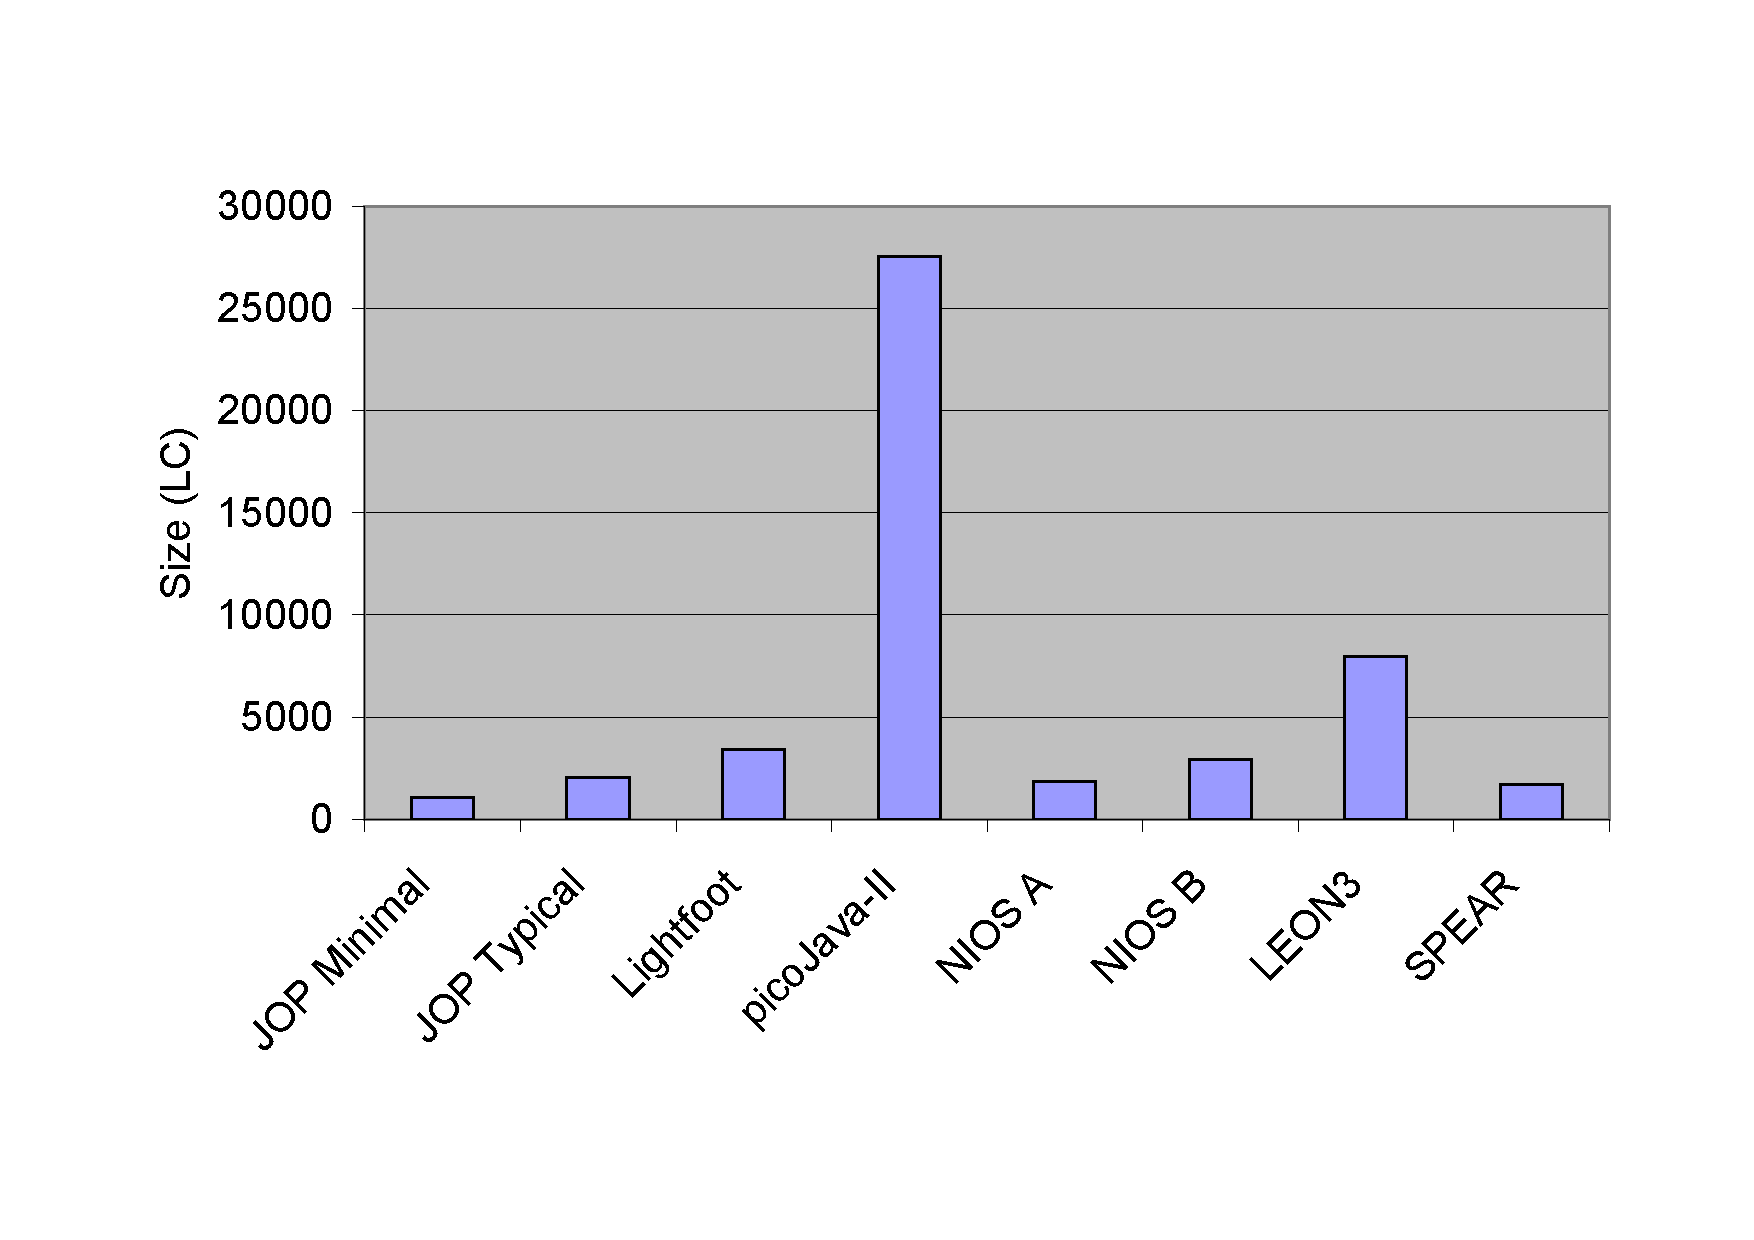
\includegraphics[width=\excelwidth]{results/size}
    \caption{Size in logic cells (LC) of different soft-core
    processors}
    \label{fig:size}
\end{figure}

One major design objective in the development of JOP was to create a
small system that can be implemented in a low-cost FPGA.
Figure~\ref{fig:size} and \tablename~\ref{tab_results_compare} show
the resource usage for different configurations of JOP and different
soft-core processors implemented in an Altera EP1C6 FPGA
\cite{AltCyc}. Estimating equivalent gate counts for designs in an
FPGA is problematic. It is therefore better to compare the two basic
structures, Logic Cells (LC) and embedded memory blocks. The maximum
frequency for all soft-core processors is in the same technology or
normalized (SPEAR) to the technology.

All configurations of JOP contain the on-chip microcode memory, the
1~KB stack cache, a 1~KB method cache, a memory interface to a
32-bit static RAM, and an 8-bit FLASH interface for the Java program
and the FPGA configuration data. The minimum configuration
implements multiplication and the shift operations in microcode. In
the typical configuration, these operations are implemented as a
sequential Booth multiplier and a single-cycle barrel shifter. The
typical configuration also contains some useful I/O devices such as
an UART and a timer with interrupt logic for multi-threading. The
typical configuration of JOP consumes about 30\% of the LCs in a
Cyclone EP1C6, thus leaving enough resources free for
application-specific logic.

As a reference, NIOS \cite{NIOS}, Altera's popular RISC soft-core, is
also included in \tablename~\ref{tab_results_compare}. NIOS has a
16-bit instruction set, a 5-stage pipeline and can be configured with
a 16 or 32-bit datapath. Version A is the minimum configuration of
NIOS. Version B adds an external memory interface, multiplication
support, and a timer. Version A is comparable with the minimal
configuration of JOP, and Version B with its typical configuration.

LEON3 \cite{LEON}, the open-source implementation of the SPARC V8
architecture, has been ported to the exact same hardware that was
used for the JOP numbers. LEON3 is representative for a RISC
processor that is used in embedded real-time systems (e.g., by ESA
for space missions).

\begin{table}
    \centering
    \begin{tabular}{lD{.}{.}{1}D{.}{.}{1.2}D{.}{.}{1}}
        \toprule
        Processor & Resources & \multicolumn{1}{c}{Memory} & \multicolumn{1}{c}{fmax} \\
                  &  (LC)    &  \multicolumn{1}{c}{(KB)} &  \multicolumn{1}{c}{(MHz)} \\
        \midrule

        JOP Minimal & 1077 & 3.25 & 98 \\
        JOP Typical & 2049 & 3.25 & 100 \\
        Lightfoot\footnotemark \cite{Lightfoot} & 3400 & 4 & 40 \\
        picoJava-II \cite{pjfpga} & 27543 & 47.6 & 43 \\
        NIOS A \cite{NIOS} & 1828 & 6.2 & 120 \\
        NIOS B \cite{NIOS} & 2923 & 5.5 & 119 \\
        LEON3 \cite{LEON} & 7978 & 10.9 & 35 \\
        SPEAR\footnotemark \cite{Delvai:ECRTS2003} & 1700 & 8 & 80 \\
        \bottomrule
    \end{tabular}
    \caption{Size and maximum frequency of FPGA soft-core processors}
    \label{tab_results_compare}
\end{table}

\addtocounter{footnote}{-1} \footnotetext{The data for the Lightfoot
processor is taken from the data sheet \cite{Lightfoot}. The
frequency used is that in a Virtex-II device from Xilinx. JOP can be
clocked at 100~MHz in the Virtex-II device, making this comparison
valid.}

\stepcounter{footnote} \footnotetext{As SPEAR uses internal memory
blocks in asynchronous mode it is not possible to synthesize it
without modification for the Cyclone FPGA. The clock frequency of
SPEAR in an Altera Cyclone is an estimate based on following facts:
SPEAR can be clocked at 40~MHz in an APEX device and JOP can be
clocked at 50~MHz in the same device.}

SPEAR \cite{Delvai:ECRTS2003} (Scalable Processor for Embedded
Applications in Real-time Environments) is a 16-bit processor with
deterministic execution times. SPEAR contains predicated
instructions to support single-path programming
\cite{Puschner:WORDS2005}. SPEAR is included in the list as it is
also a processor designed for real-time systems.

To prove that the VHDL code for JOP is as portable as possible, JOP
was also implemented in a Xilinx Spartan-3 FPGA \cite{Spartan3}.
Only the instantiation and initialization code for the on-chip
memories is vendor-specific, whilst the rest of the VHDL code can be
shared for the different targets. JOP consumes about the same LC
count (1844~LCs) in the Spartan device, but has a slower clock
frequency (83~MHz).

From this comparison we can see that we have achieved our objective
of designing a small processor. The commercial Java processor,
Lightfoot, consumes 1.7 times the logic resources of JOP in the
typical configuration (with a lower clock frequency). A typical
32-bit RISC processor (NIOS) consumes about 1.5 times (LEON about
four times) the resources of JOP. However, the NIOS processor can be
clocked 20\% faster than JOP in the same technology. The vendor
independent and open-source RISC processor LEON can be clocked only
with 35\% of JOP's frequency. The only processor that is similar in
size is SPEAR. However, while SPEAR is a 16-bit processor, JOP
contains a 32-bit datapath.


%\begin{table}
%    \centering
%    \begin{tabular}{llrr}
%        \toprule
%        JOP & Optimization & Resource [LC] & fmax [MHz] \\
%        \midrule
%        Typical (iomin) & default & 1930 & 101 \\
%         & Reg.pack: min. Area w/Chains & 1764 & 99 \\
%         & + Synth. Area & 1746 & 98 \\
%         & Reg.pack: min. Are w/Chains + Synth speed & 1800
%        & 100 \\
%        Core (no io) & Reg.pack, Synth Area & 1452 & 98 \\
%        - mul & & 1296 & 99 \\
%        - shift & with single bit sar & 1077 & 98 \\
%        \midrule
%        Typical, Spartan-3 & speed & 1844 & 83 \\
%        Typical, Spartan-3 & area & 1689 & 74 \\
%        \bottomrule
%    \end{tabular}
%    \caption{FPGA Soft Core Processors}
%    \label{tab_results_jop_versions}
%\end{table}

%Different LC/gate values:
%    from tow-level stack: 1LC = 5.4 gates
%    from ram stack: 1LC = 5.5 gates
%    from register stack: 1LC = 5.9 gates
%    Moon: 3660LCs - 27K gates + 3KB ROM + 1KB RAM: 1LC = 7.4 gates
%    Lightfoot: 3400LCs - 25K gates: 1LC = 7.4 gates
%    picoJava: ROM/RAM - 1Bit = 1 gate
%
%    JOP: 1831 LCs, 3.25KB: 1831*6 + 26624*1.5 = 11K + 39k
%    JOP: 2050*6 + 3.5*1024*8*1.5 = 12K + 43K
%    Pentium MMX: 4.5 Mio. Transistors -> 1100K

Table~\ref{tab:results:gate:count} provides gate count estimates for
JOP, picoJava, the aJile processor, and the Intel Pentium MMX
processor that is used in the benchmarks in the next section.
Equivalent gate count for an LC\footnote{The factors are derived
from the data provided for various processors in
Chapter~\ref{chap:related} and from the resource estimates in
Section~\ref{sec:stack}.} varies between 5.5 and 7.4 -- we chose a
factor of 6 gates per LC and 1.5 gates per memory bit for the
estimated gate count for JOP in the table. JOP is listed in the
typical configuration that consumes 2050 LCs. The Pentium MMX
contains 4.5M transistors \cite{pentium:mmx} that are equivalent to
1125K gates.

\begin{table}
    \centering
    \begin{tabular}{lrrr}
        \toprule
        Processor & \multicolumn{1}{c}{Core} & \multicolumn{1}{c}{Memory} & \multicolumn{1}{c}{Sum.} \\
        & \multicolumn{1}{c}{[gate]} & \multicolumn{1}{c}{[gate]} & \multicolumn{1}{c}{[gate]}\\
        \midrule
        JOP & 12K & 43K & 55K\\
        picoJava & 128K & 314K & 442K\\
        aJile & 25K & 912K & 937K\\
        Pentium MMX & & & 1125K\\
        \bottomrule
    \end{tabular}
    \caption{Gate count estimates for various processors}
    \label{tab:results:gate:count}
\end{table}

We can see from the table that the on-chip memory dominates the
overall gate count of JOP, and to an even greater extent, of the
aJile processor. The aJile processor is roughly the same size as the
Pentium MMX, and both are about 20 times larger than JOP.


\section{Performance}
\label{sec:performance}

In this section, we will evaluate the performance of JOP in relation
to other Java systems. Although JOP is intended as a processor with
a low WCET for all operations, its general performance is still
important. In the first section, we will evaluate JOP's average
performance.

%In the section that follows it, the implementation of the simple
%real-time profile, as described in Section~\ref{sec:rtprof}, on JOP
%is compared to the RI of the RTSJ on top of Linux.

The comparison of the implementation of the simple real-time profile,
as described in Section~\ref{sec:rtprof}, on JOP with the RI of the
RTSJ on top of Linux can be found in \cite{jop:rtjava}.

\subsection{General Performance}

Running benchmarks is problematic, both generally and especially in
the case of embedded systems. The best benchmark would be the
application that is intended to run on the system being tested. To
get comparable results, SPEC provides benchmarks for various systems.
However, the one for Java, the SPECjvm98 \cite{SPECJvm98}, needs more
functionality than what is usually available in a CLDC compliant
device (e.g., a filesystem and \code{java.net}). Some benchmarks from
the SPECjvm98 suites also need several megabaytes of heap.

Due to the absence of a \emph{standard} Java benchmark for embedded
systems, a small benchmark suite that should run on even the
smallest device is provided here. It contains several
micro-benchmarks for evaluating the number of clock cycles for
single bytecodes or short sequences of bytecodes, and two
application benchmarks.

To provide a realistic workload for embedded systems, a real-time
application was adapted to create the first application benchmark
(Kfl). The application is taken from one of the nodes of a
distributed motor control system \cite{jop:wises03} (the first
industrial application of JOP). The application is written as a
cyclic executive. A simulation of both the environment (sensors and
actors) and the communication system (commands from the master
station) forms part of the benchmark, so as to simulate the
real-world workload. The second application benchmark is an
adaptation of a tiny TCP/IP stack for embedded Java. This benchmark
contains two UDP server/clients, exchanging messages via a loopback
device. The Kfl benchmark consists of 511 methods and 14~KB code,
the UDP/IP benchmark of 508 methods and 13~KB code (including the
supporting library).

As we will see, there is a great variation in processing power
across different embedded systems. To cater for this variation, all
benchmarks are `self adjusting'. Each benchmark consists of an
aspect that is benchmarked in a loop and an `overhead' loop that
contains any overheads from the benchmark that should be subtracted
from the result (this feature is designed for the micro-benchmarks).
The loop count adapts itself until the benchmark runs for more than
a second. The number of iterations per second is then calculated,
which means that higher values indicate better performance.

%Teilweise Wiederholung

All the benchmarks measure how often a function is executed per
second. In the Kfl benchmark, this function contains the main loop of
the application that is executed in a periodic cycle in the original
application. In the benchmark, the wait for the next period is
omitted, so that the time measured solely represents execution time.
The UDP benchmark contains the generation of a request, transmitting
it through the UDP/IP stack, generating the answer and transmitting
it back as a benchmark function. The iteration count is the number of
received answers per second.

The accuracy of the measurement depends on the resolution of the
system time. For the measurements under Linux, the system time has a
resolution of 10ms, resulting in an inaccuracy of 1\%. The accuracy
of the system time on leJOS, TINI and the aJile is not known, but is
considered to be in the same range. For JOP, a $\mu$s counter is
used for time measurement.


The following list gives a brief description of the Java systems
that were benchmarked:

\begin{description}
    \item[JOP]
is implemented in a Cyclone FPGA \cite{AltCyc}, running at 100~MHz.
The main memory is a 32-bit SRAM (15ns) with an access time of 2
clock cycles. The benchmarked configuration of JOP contains a 4~KB
method cache organized in 16 blocks.

    \item[leJOS] As an example for a low-end embedded device, we
        use the RCX robot controller from the LEGO MindStorms
        series. It contains a 16-bit Hitachi H8300
        microcontroller \cite{hitachi:h8}, running at 16~MHz.
        leJOS \cite{lejos} is a tiny interpreting JVM for the
        RCX.

    \item[KVM] is a port of Sun's KVM, is part of the Connected
        Limited Device Configuration (CLDC) \cite{J2ME}, to
        Altera's NIOS II processor on MicroC Linux. NIOS is
        implemented on a Cyclone FPGA and clocked at 50~MHz.
        Besides the different clock frequency, this is a good
        comparison of an interpreting JVM running in the same
        FPGA as JOP.

    \item[TINI]
is an enhanced 8051 clone running a software JVM. The results were
taken from a custom board with a 20~MHz crystal, and the chip's PLL
is set to a factor of 2.

    \item[Cjip]
The measured system \cite{SNAP} is a replacement of the TINI board
and contains a Cjip \cite{Cjip} clocked with 80~MHz and 8~MB DRAM.

    \item[Komodo]
Komodo \cite{komodo2003} is a Java processor as a basis for research
on real-time scheduling on a multithreaded microcontroller (see
Section~\ref{subsec:related:komodo}). The benchmark results were
obtained by Matthias Pfeffer \cite{Pfeffer} on a cycle-accurate
simulation of Komodo. The values are obtained without garbage
collection. According to Pfeffer, Komodo can be clocked with 33MHz
in a Xlinix XCV800.

    \item[aJile] aJile's JEMCore is a direct-execution Java
        processor that is available in two different versions:
        the \textbf{aJ80} and the \textbf{aJ100} \cite{aJile}.
        The aJ100 provides a generic 8-bit, 16-bit, or 32-bit
        external bus interface, while the aJ80 only provides an
        8-bit interface.


    \item[EJC]
The Embedded Java Controller (EJC) platform \cite{EJC} is a typical
example of a JIT system on a RISC processor. The system is based on
a 32-bit ARM720T processor running at 74~MHz. It contains up to
64~MB SDRAM and up to 16~MB of NOR flash.

    \item[gcj]
is the GNU compiler for Java. This configuration represents the
batch compiler solution, running on a 266~MHz Pentium MMX under
Linux.

    \item[MB]
is the realization of Java on a RISC processor for an FPGA (Xilinx
MicroBlaze \cite{microblaze}). Java is compiled to C with a Java
compiler for real-time systems \cite{Java2C} and the C program is
compiled with the standard GNU toolchain.

\end{description}

It would be interesting to include the other soft-core Java
processors (Moon, Lightfoot, and FemtoJava) in this comparison.
However, it was not possible to obtain the benchmark data. The
company that produced Moon seems to have disappeared and FemtoJava
could not run all benchmarks.


\begin{figure}
    \centering
    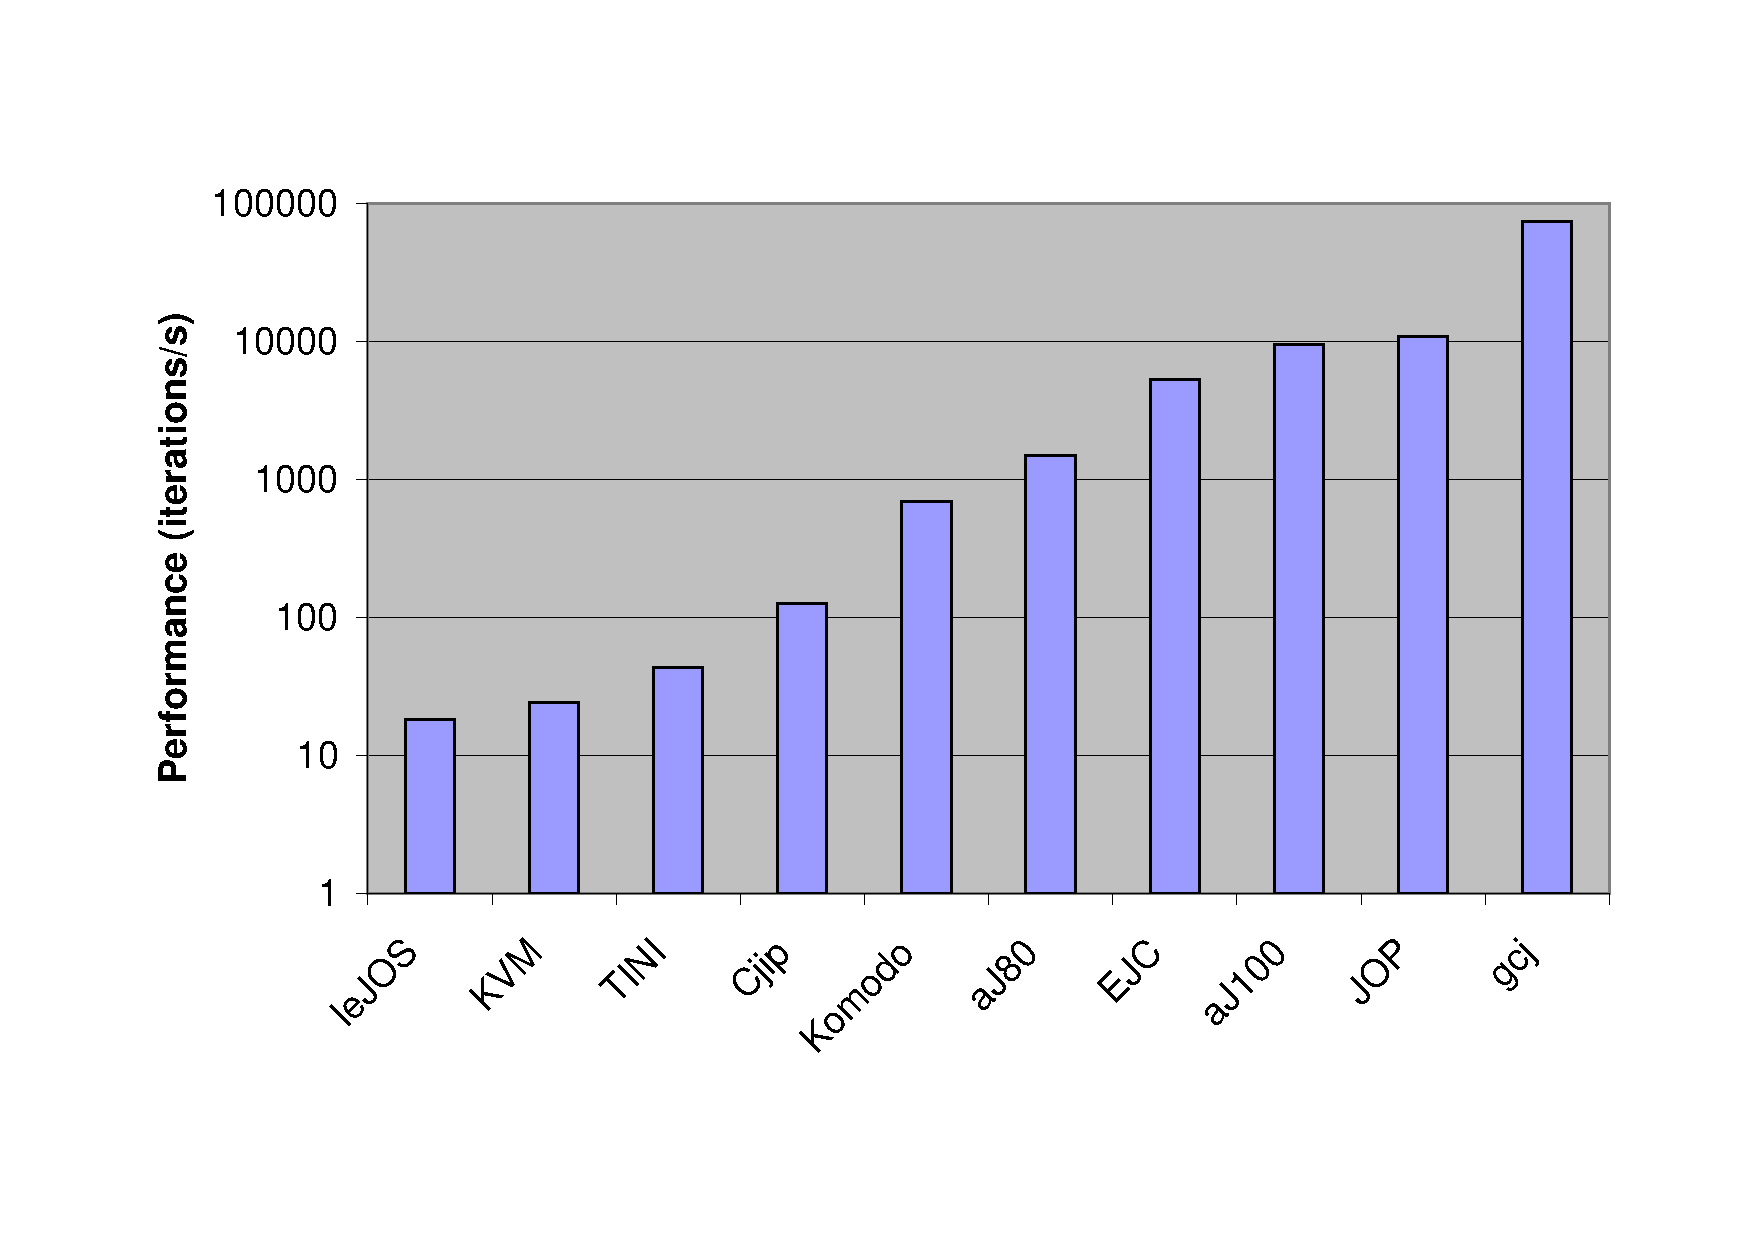
\includegraphics[width=\excelwidth]{results/results_app_bench}
    \\
    \vspace{0.5cm}
    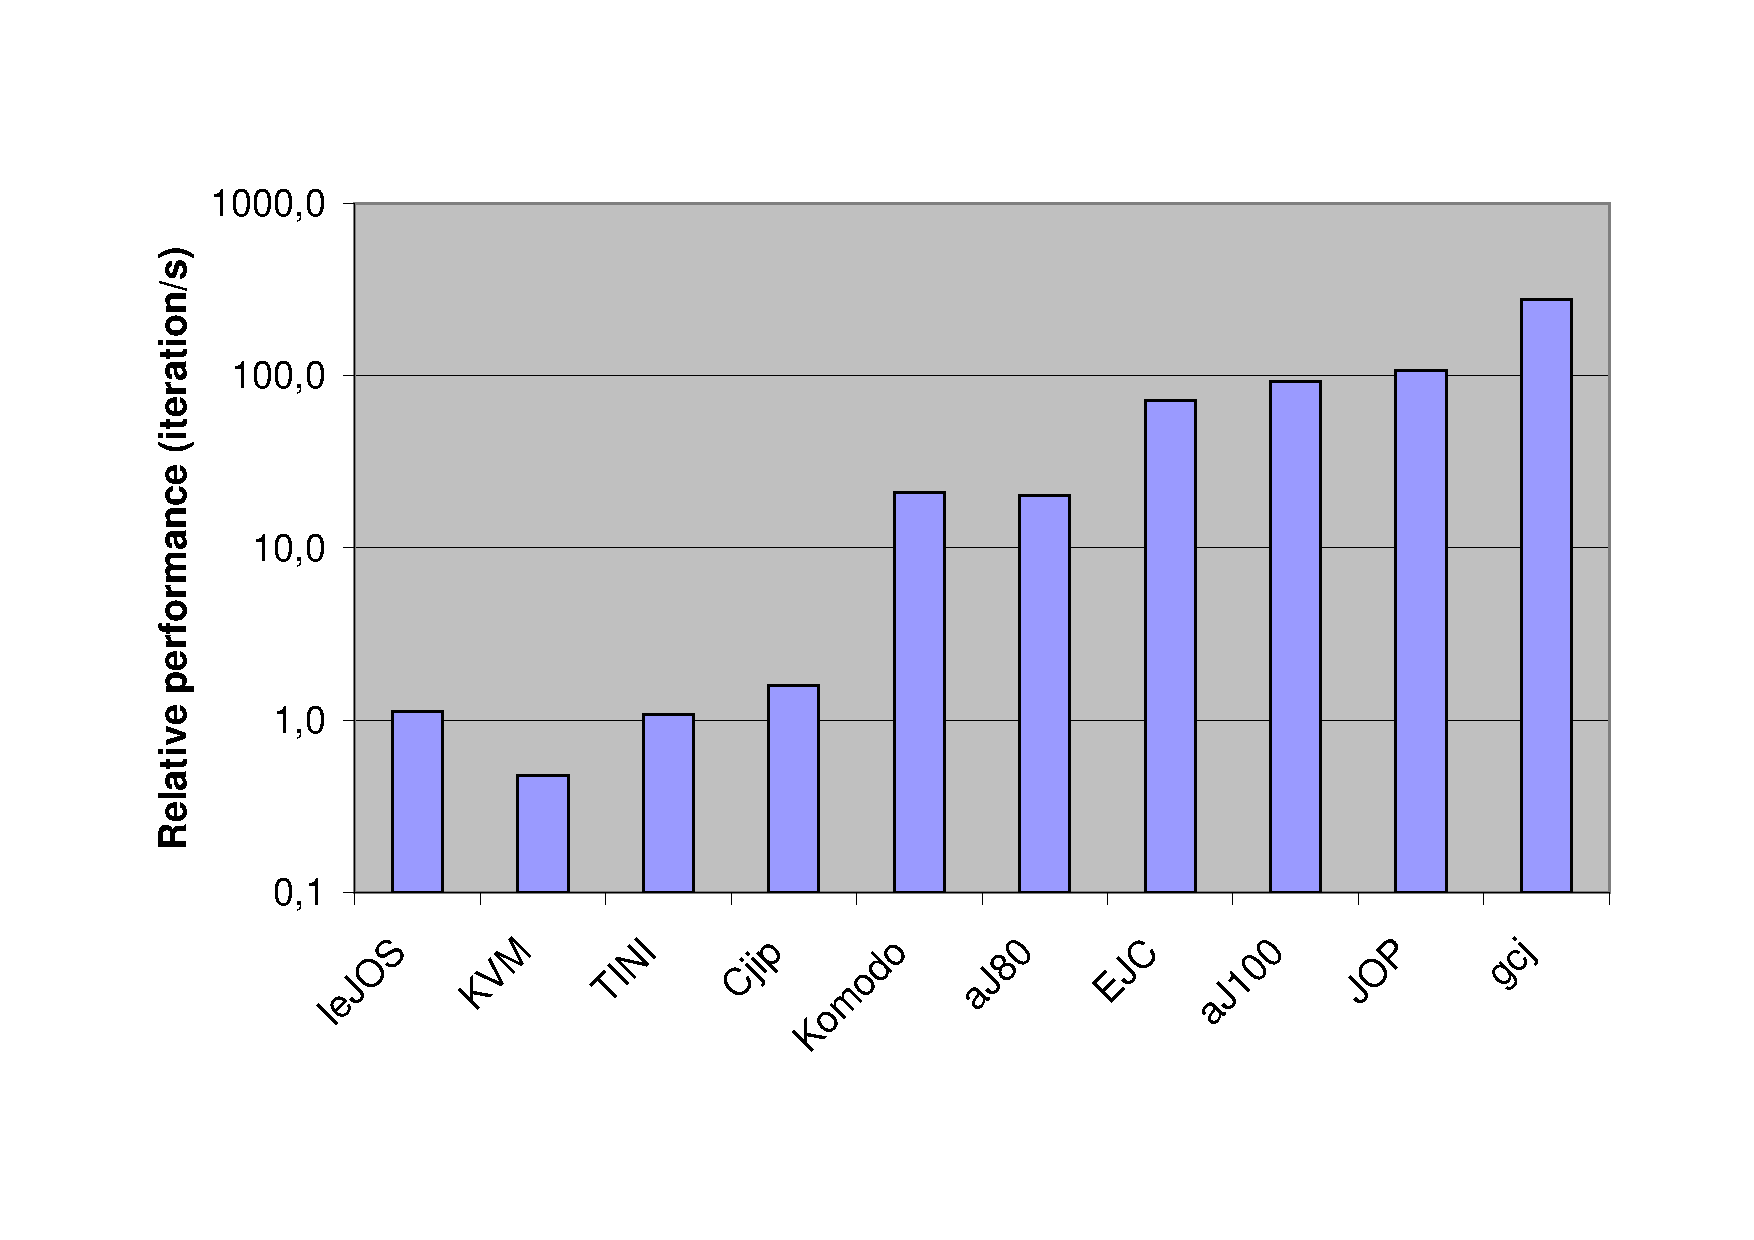
\includegraphics[width=\excelwidth]{results/results_app_bench_scaled}
    \caption{Performance comparison of different Java systems with
    application benchmarks. The diagrams show the geometric mean
    of the two benchmarks in iterations per second -- a higher
    value means higher performance. The top diagram shows
    absolute performance, while the bottom diagram shows the result
    scaled to 1~MHz clock frequency.
    }
    \label{fig:results:app:bench}
\end{figure}


In Figure~\ref{fig:results:app:bench}, the geometric mean of the two
application benchmarks is shown. The unit used for the result is
iterations per second. Note that the vertical axis is logarithmic,
in order to obtain useful figures to show the great variation in
performance. The top diagram shows absolute performance, while the
bottom diagram shows the same results scaled to a 1~MHz clock
frequency. The results of the application benchmarks and the
geometric mean are shown in \tablename~\ref{tab:results:bench:app}.


It should be noted that scaling to a single clock frequency could
prove problematic. The relation between processor clock frequency
and memory access time cannot always be maintained. To give an
example, if we were to increase the results of the 100~MHz JOP to
1~GHz, this would also involve reducing the memory access time from
15~ns to 1.5~ns. Processors with 1~GHz clock frequency are already
available, but the fastest asynchronous SRAM to date has an access
time of 10~ns.

%To compare the performance relatively to the size of the different
%systems, Figure~\ref{fig:results:app:bench:double:scaled} shows the
%performance of JOP, the aJ100 and the gcj PC versions relative to
%the gate count (from Table~\ref{tab:results:gate:count}) and clock
%frequency. Relative to size and clock frequency, JOP outperforms the
%aJile processor by a factor of 20 and even the gcj-compiler on the
%Pentium MMX by a factor of 8.





\begin{table}
    \centering
    \begin{tabular*}{\columnwidth}{@{\extracolsep{\fill}}lD{.}{.}{2}rrD{.}{.}{2}D{.}{.}{2}}
%    \begin{tabular}{lrrrrrr}
        \toprule

 & \multicolumn{1}{c}{Frequency} & \multicolumn{1}{c}{Kfl} & \multicolumn{1}{c}{UDP/IP}
    & \multicolumn{1}{c}{Geom. Mean} & \multicolumn{1}{c}{Scaled}\\
 &  \multicolumn{1}{c}{(MHz)} &  \multicolumn{4}{c}{(Iterations/s)}\\
        \midrule
JOP & 100 & 17111 & 6781 & 10772 & 108\\
leJOS & 16 & 25 & 13 & 18 & 1.1\\
TINI & 40 & 64 & 29 & 43 & 1.1\\
KVM & 50 & 36 & 16 & 24 & 0.5\\
Cjip & 80 & 176 & 91 & 127 & 1.6\\
Komodo & 33 & 924 & 520 & 693 & 21\\
aJ80 & 74 & 2221 & 1004 & 1493 & 20\\
aJ100 & 103 & 14148 & 6415 & 9527 & 92\\
EJC & 74 & 9893 & 2822 & 5284 & 71\\
%Sun jvm & 266 & 212,952 & 91,851 & 139,857 & 526\\
gcj & 266 & 139884 & 38460 & 73348 & 276\\
%Xint & 266 & 17,310 & 8,747 & 12,305 & 46\\
MB & 100 & 3792 &  &  & \\
% MB 8KB/8KB & 100 & 25,090 &  &  & \\
        \bottomrule

    \end{tabular*}
    \caption{Application benchmarks on different Java systems.
    The table shows the benchmark results in
    iterations per second -- a higher
    value means higher performance.
    }
    \label{tab:results:bench:app}
\end{table}

% not
%\begin{figure}
%    \centering
%    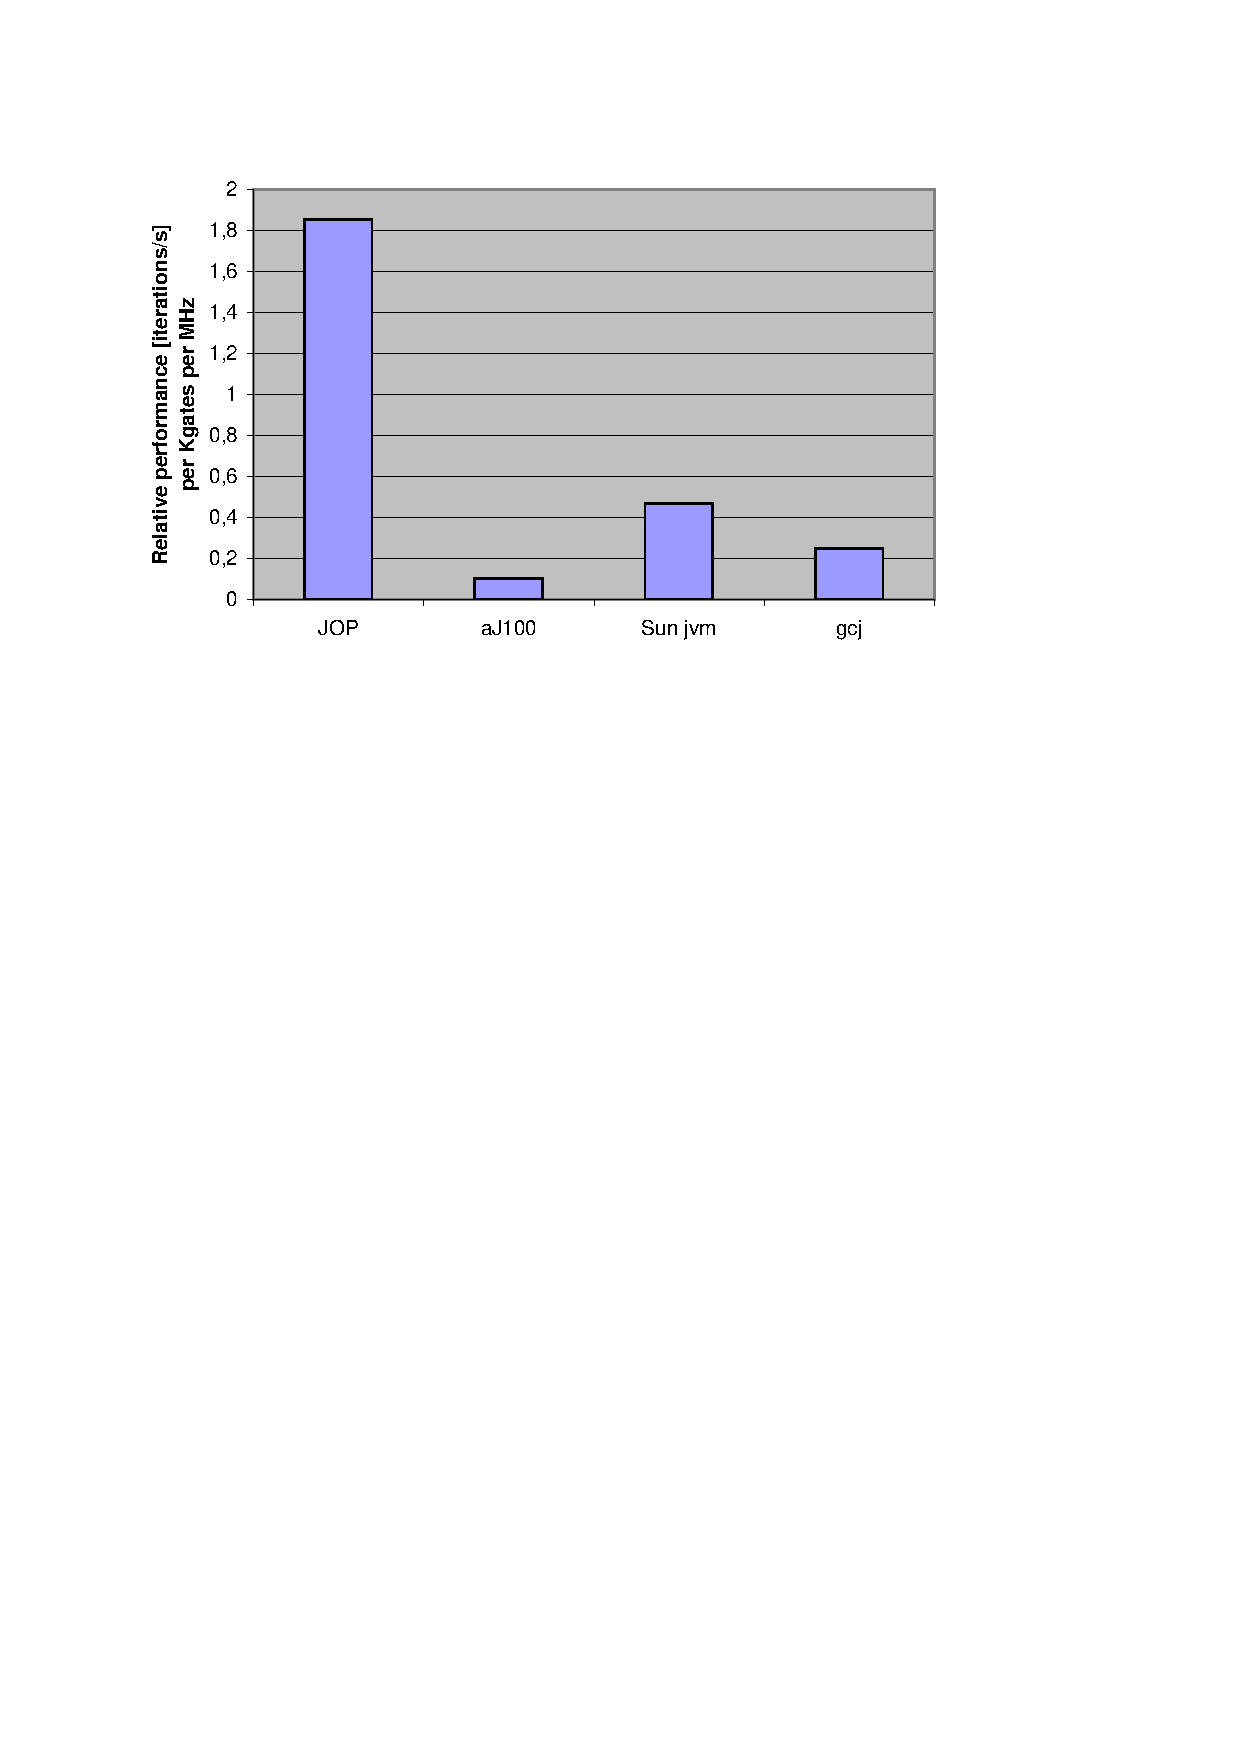
\includegraphics[width=\excelwidth]{results_app_bench_double_scaled}
%    \caption{Performance comparison of different Java systems with
%    application benchmarks. The diagram shows the result scaled to
%    the chip size (Kgates) and clock frequency (MHz).
%    }
%    \label{fig:results:app:bench:double:scaled}
%\end{figure}


\subsection{Discussion}
\label{sec:perf:disc}

When comparing JOP and the aJile processor against leJOS, KVM, and
TINI, we can see that a Java processor is up to 500 times faster
than an interpreting JVM on a standard processor for an embedded
system. The average performance of JOP is even better than a
JIT-compiler solution on an embedded system, as represented by the
EJC system.

Even when scaled to the same clock frequency, the compiling JVM on a
PC (gcj) is much faster than either embedded solution. However, the
kernel of the application is smaller than 4~KB
\cite{jop:jtres_cache}. It therefore fits in the level one cache of
the Pentium MMX. For a comparison with a Pentium class processor we
would need a larger application.

JOP is about 7 times faster than the aJ80 Java processor on the
popular JStamp board. However, the aJ80 processor only contains an
8-bit memory interface, and suffers from this bottleneck. The SaJe
system contains the aJ100 with 32-bit, 10~ns SRAMs. JOP with its
15~ns SRAMs is about 12\% faster than the aJ100 processor.

The MicroBlaze system is a representation of a Java batch-compilation
system for a RISC processor. MicroBlaze is configured with the same
cache\footnote{The MicroBlaze with an 8~KB data and 8~KB instruction
cache is about 1.5 times faster than JOP. However, a 16~KB memory is
not available in low-cost FPGAs and is an unbalanced system with
respect to the LC/memory relation.} as JOP and clocked at the same
frequency. JOP is about four times faster than this solution, thus
showing that native execution of Java bytecodes is faster than
batch-compiled Java on a similar system. However, the results of the
MicroBlaze solution are at a preliminary stage\footnote{As not all
language constructs can be compiled, only the Kfl benchmark was
measured. Therefore, the bars for MicroBlaze are missing in
\figurename~\ref{fig:results:app:bench}.}, as the Java2C compiler
\cite{Java2C} is still under development.

The micro-benchmarks are intended to give insight into the
implementation of the JVM. In Table~\ref{tab:results:bench:clock},
we can see the execution time in clock cycles of various bytecodes.
As almost all bytecodes manipulate the stack, it is not possible to
measure the execution time for a single bytecode in the benchmark
loop. The single bytecode would trash the stack. As a minimum
requirement, a second instruction is necessary in the loop to
reverse the stack operation.

\begin{table}
    \centering
    \begin{tabular*}{\columnwidth}{@{\extracolsep{\fill}}lrrrrrrrr}
        \toprule

                      & JOP & leJOS & TINI  & Cjip & Komodo & aJ80 & aJ100 \\
        \midrule
    iload iadd         & 2 & 836 & 789      & 55 & 8 & 38 & 8 \\
    iinc               & 8 & 422 & 388      & 46 & 4 & 41 & 11 \\
    ldc                & 9 & 1340 & 1128  & 670 & 40 & 67 & 9 \\
    if\_icmplt taken   & 6 & 1609 & 1265  & 157 & 24 & 42 & 18 \\
    if\_icmplt n/taken & 6 & 1520 & 1211  & 132 & 24 & 40 & 14 \\
    getfield           & 22 & 1879 & 2398 & 320 & 48 & 142 & 23 \\
    getstatic          & 15 & 1676 & 4463 & 3911 & 80 & 102 & 15 \\
    iaload             & 36 & 1082 & 1543 & 139 & 28 & 74 & 13 \\
    invoke             & 128 & 4759 & 6495& 5772 & 384 & 349 & 112 \\
    invoke static      & 100 & 3875 & 5869& 5479 & 680 & 271 & 92 \\
    invoke interface   & 144 & 5094 & 6797& 5908 & 1617 & 531 & 148 \\

        \bottomrule
    \end{tabular*}
    \caption{Execution time in clock cycles for various JVM bytecodes}
    \label{tab:results:bench:clock}
\end{table}

For JOP we can deduce that the WCET for simple bytecodes  is also the
average execution time. We can see that the combination of
\code{iload} and \code{iadd} executes in two cycles, which means that
each of these two operations is executed in a single cycle. The
\code{iinc} bytecode is one of the few instructions that does not
manipulate the stack and can be measured alone. As \code{iinc} is not
implemented in hardware, we have a total of 8 cycles that are
executed in microcode. It is fair to assume that this comprises too
great an overhead for an instruction that is found in every iterative
loop with an integer index. However, the decision to implement this
instruction in microcode was derived from the observation that the
dynamic instruction count for \code{iinc} is only 2\% (see
Section~\ref{sec:bench:jvm}).

The sequence for the branch benchmark (\code{if\_icmplt}) contains
the two load instructions that push the arguments onto the stack.
The arguments are then consumed by the branch instruction. This
benchmark verifies that a branch requires a constant four cycles on
JOP, whether it is taken or not.

The Cjip implements the JVM with a stack oriented instruction set. It
is the only example (except JOP) where the instruction set is
documented \emph{including} the execution time \cite{CjipRef}. We
will therefore check some of the results with the numbers provided in
the documentation. The execution time is given in nanoseconds,
assuming a 66~MHz clock. The execution time for the basic integer add
operation is given as 180~ns resulting in 12 cycles. The load of a
local variable (when it is one of the first four) takes 35 cycles. In
the micro-benchmark we measure 55 cycles instead of the theoretical
47 (\code{iadd} + \code{iload\_n}). We assume that we have to add
some cycles for the fetch of the bytecodes from memory.

For compiling versions of the JVM, these micro-benchmarks do not
produce useful results. The compiler performs optimizations that
make it impossible to measure execution times at this fine a
granularity.

During the evaluation of the aJile system, unexpected behavior was
observed. The aJ80 on the JStamp board is clocked at 7.3728~MHz, and
the internal frequency can be set with a PLL. The aJ80 is rated for
80MHz and the maximum PLL factor that can be used is therefore ten.
Running the benchmarks with different PLL settings gave some strange
results. For example, with a PLL multiplier setting of ten, the aJ80
was about 12.8 times faster! Other PLL factors also resulted in a
greater than linear speedup. The only explanation we could find was
that the internal time, \code{System.currentTimeMillis()}, used for
the benchmarks depends on the PLL setting. A comparison with the wall
clock time showed that the internal time of the aJ80 is 23\% faster
with a PLL factor of 1 and 2.4\% faster with a factor of ten -- a
property we would not expect on a processor that is marketed for
real-time systems.

The SaJe board is also clocked with 7.3728~MHz and the PLL factor is
set to 14. This gives a 103.2192~MHz internal clock frequency.
However, it is not known how accurate the internal time is in this
setting. The results for the SaJe board can also suffer from the
problem described above.

% aJ80 at 7.3728MHz: internal 11' are external 8'57'' ... 1.23 times too fast
% aJ80 at 73.728MHz: internal 21' are external 20'30'' ... 1.024 times too fast




\subsection{Execution Time Jitter}

For real-time systems, the worst-case of the execution time is of
primary importance. We have measured the execution times of several
iterations of the main function from the Kfl benchmark.
\figurename~\ref{fig:results:kfl:exe} shows the measurements, scaled
to the minimum execution time.

\begin{figure}
    \centering
    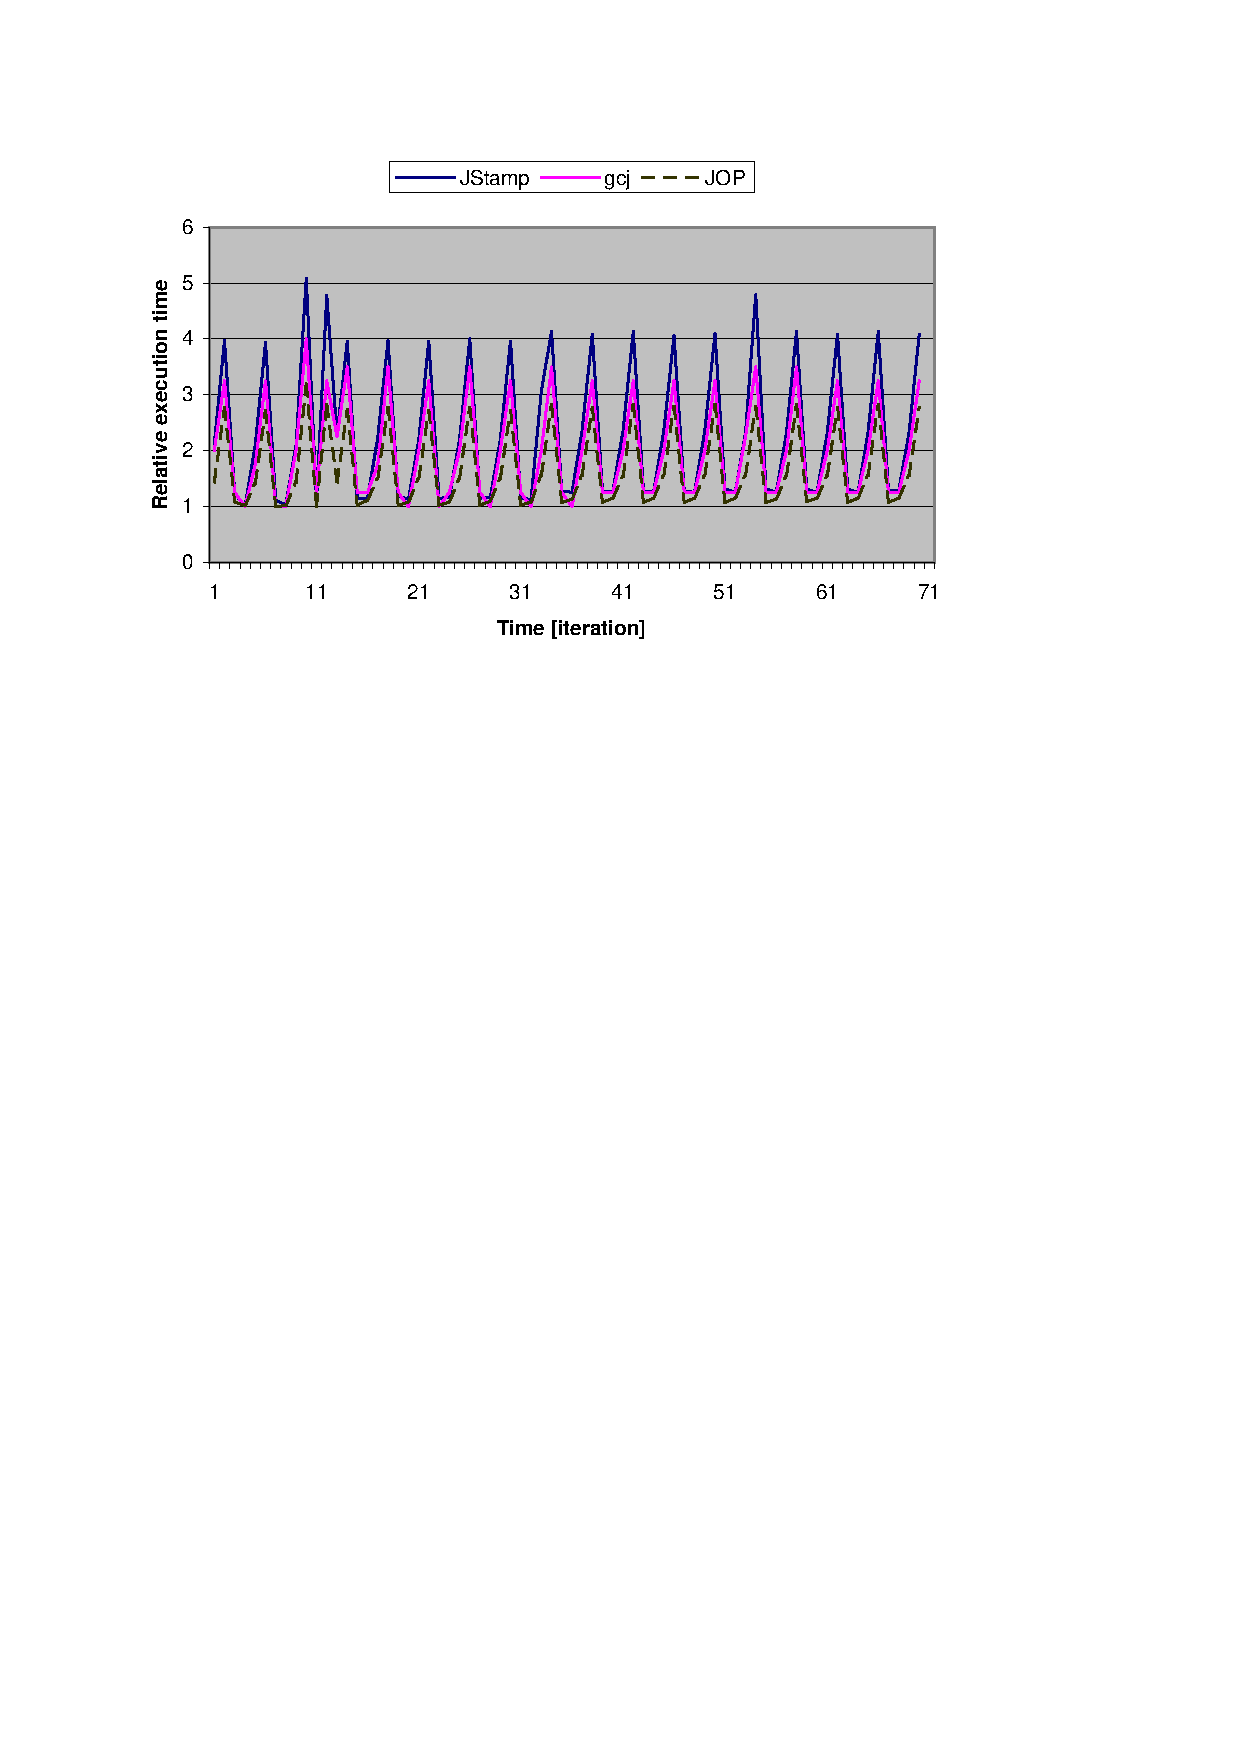
\includegraphics[width=\excelwidth]{results/results_kfl_exe}
    \\
    \vspace{0.5cm}
    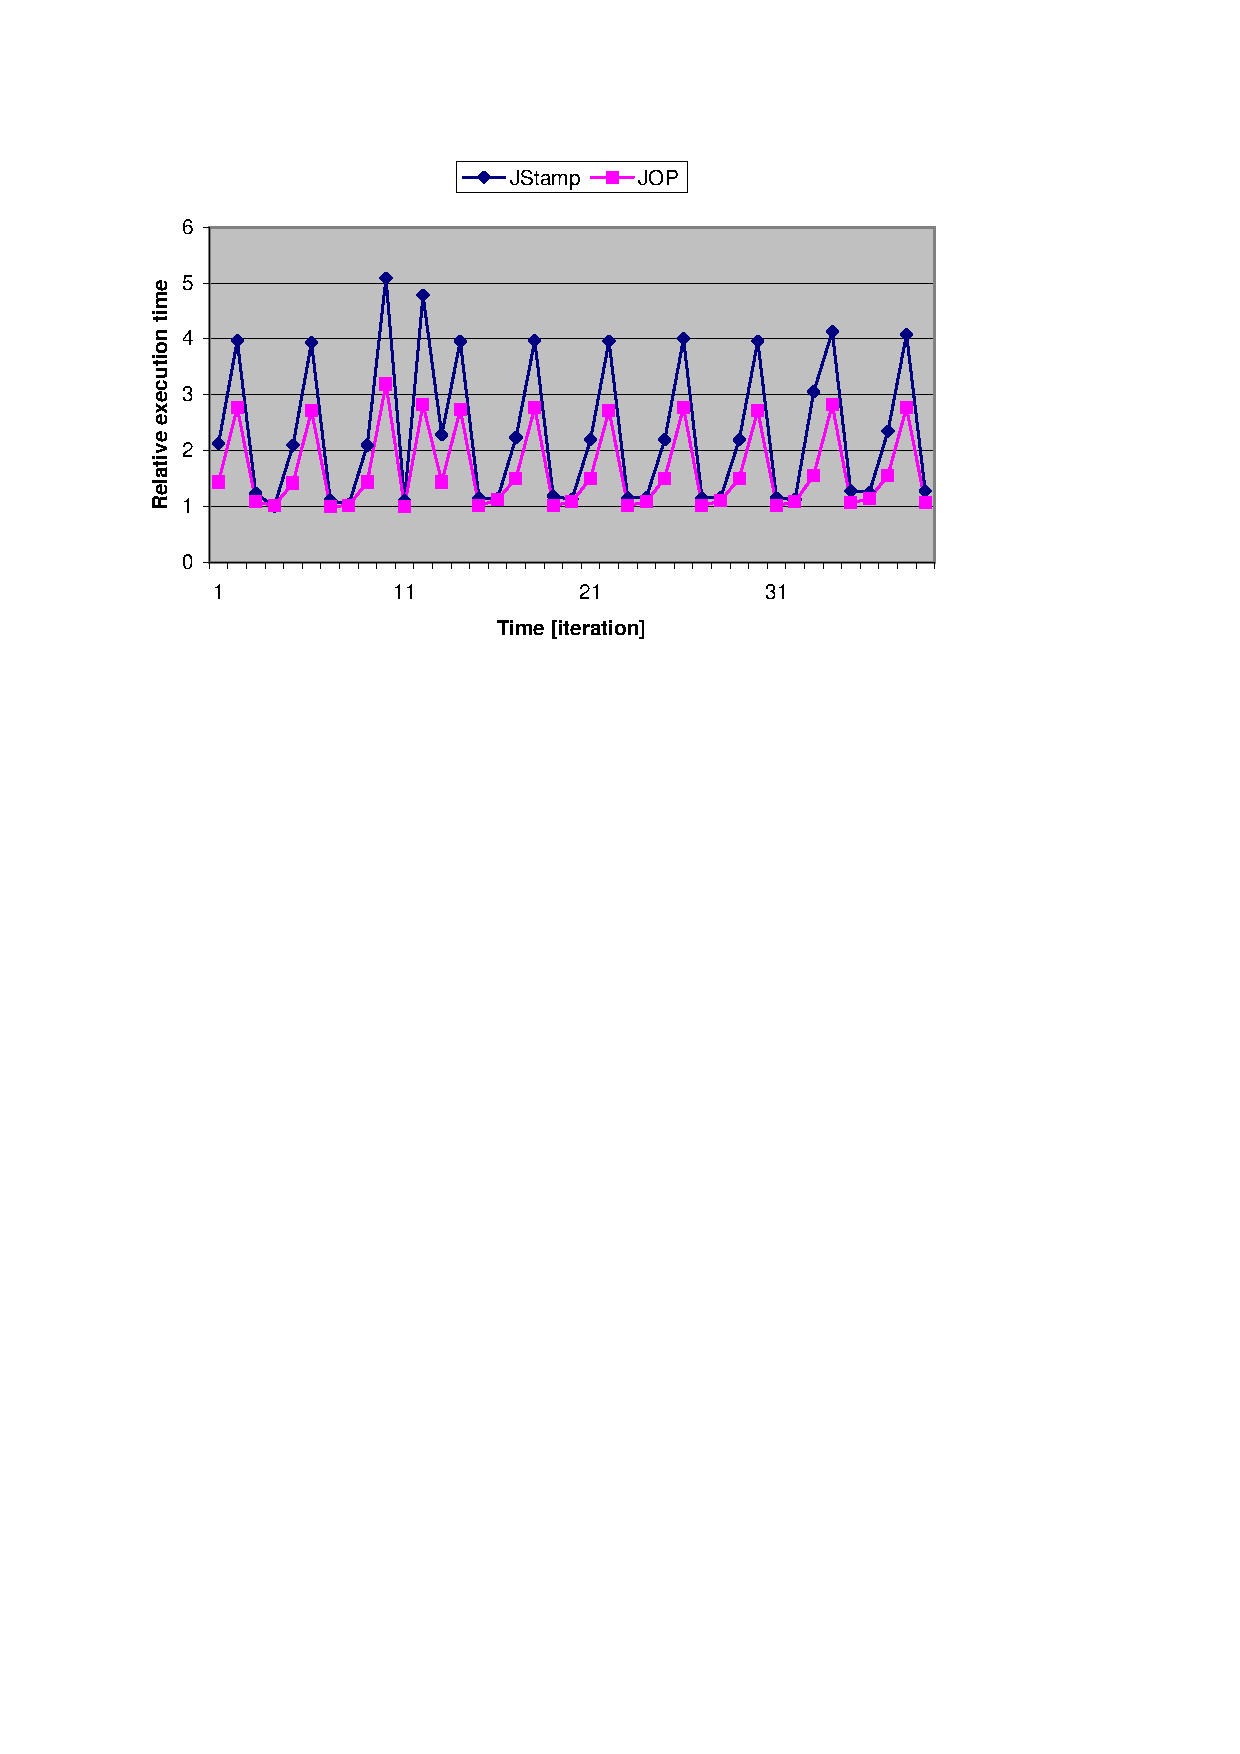
\includegraphics[width=\excelwidth]{results/results_kfl_exe_detail}
    \caption{Execution time of the main function for the Kfl benchmark.
    The values are scaled to the minimum execution time. The bottom
    figure shows a detail of the top figure.
    }
    \label{fig:results:kfl:exe}
\end{figure}

%\begin{figure}
%    \centering
%    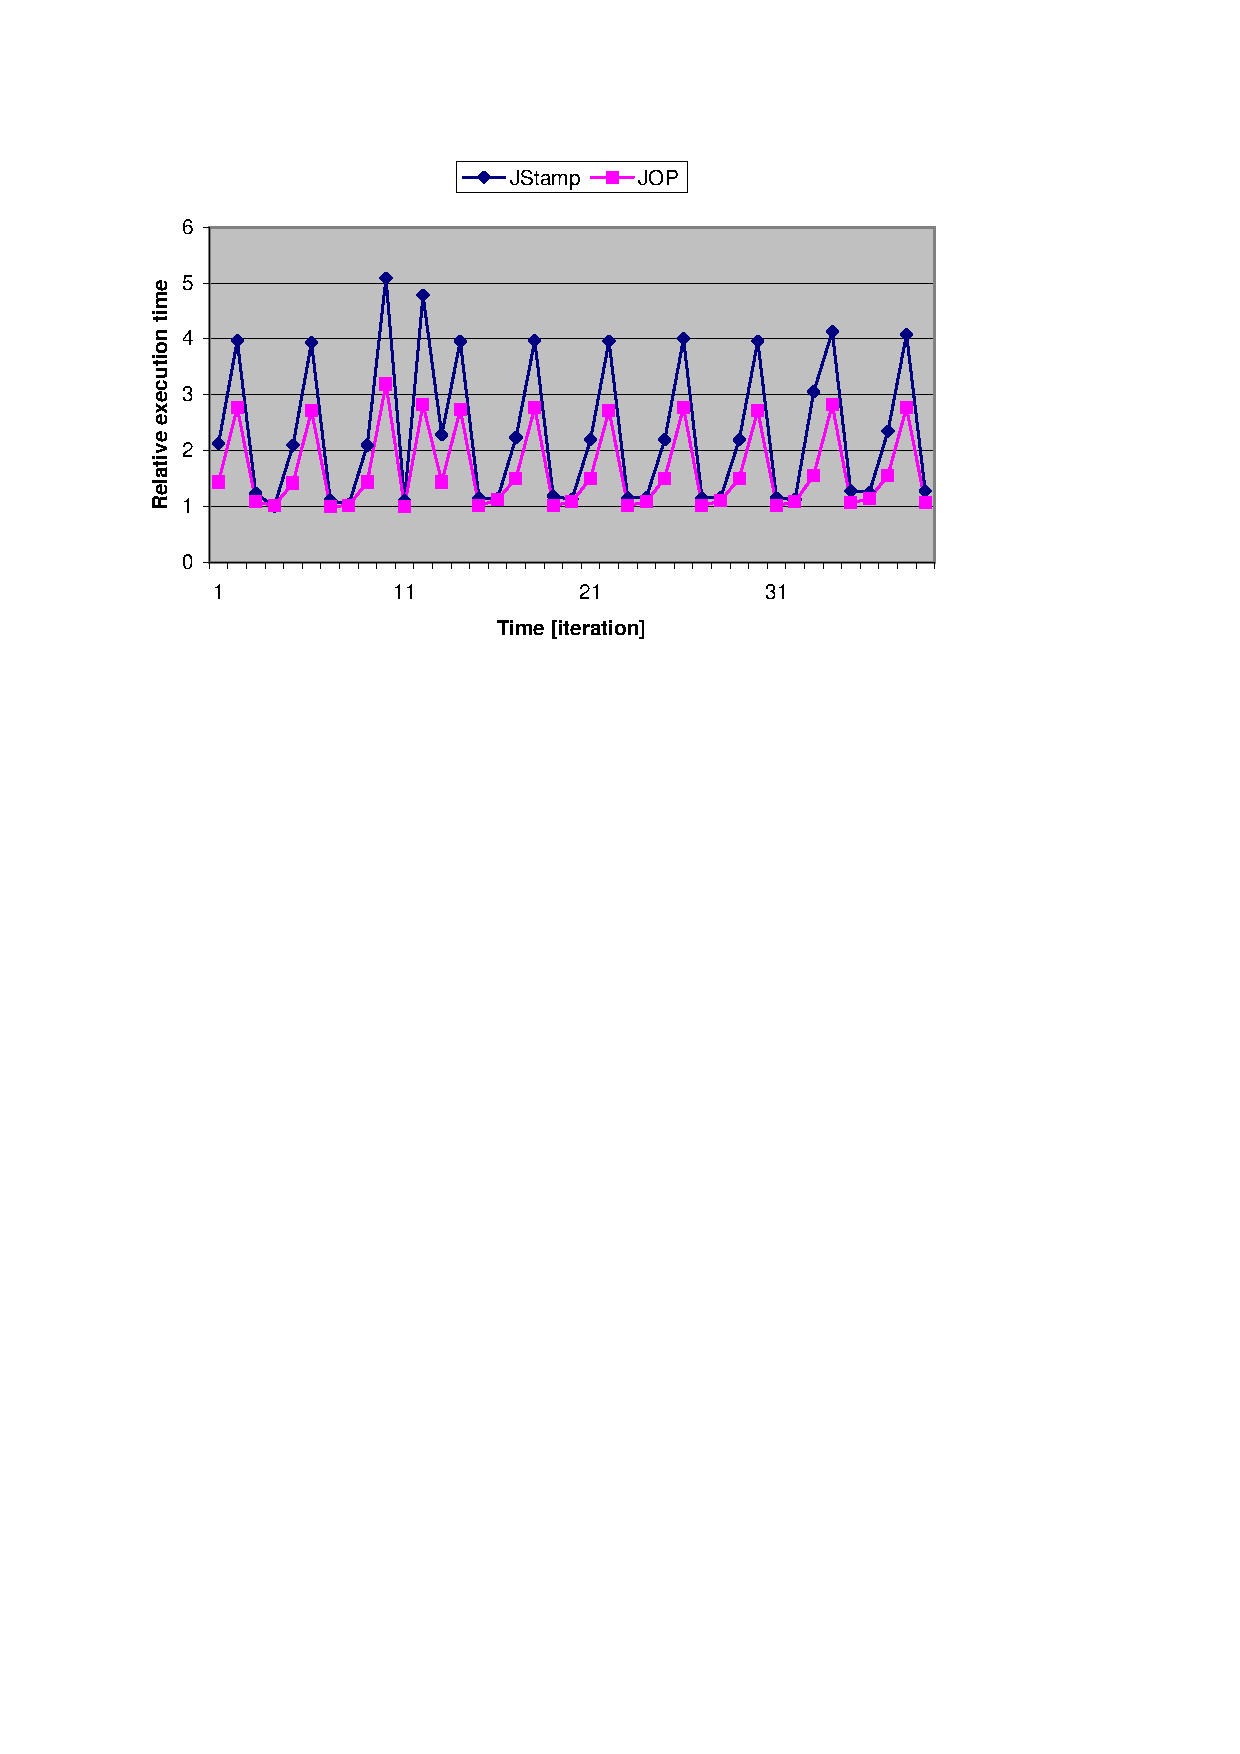
\includegraphics{results/results_kfl_exe_detail}
%    \caption{Execution time with KFL benchmark (detail).}
%    \label{fig:results:kfl:exe:detail}
%\end{figure}

A period of four iterations can be seen. This period results from
simulating the commands from the base station that are executed
every fourth iteration. At iteration 10, a command to start the
motor is issued. We see the resulting rise in execution time at
iteration 12 to process this command. At iteration 54, the
simulation triggers the end sensor and the motor is stopped.

The different execution times in the different modes of the
application are inherent in the design of the simulation. However,
the ratio between the longest and the shortest period is five for the
JStamp, four for the gcj system, and only three for JOP. Therefore, a
system with an aJile processor needs to be 1.7 times faster than JOP
in order to provide the same WCET for this measurement. At iteration
33, we can see a higher execution time for the JStamp system that is
not seen on JOP. This variation at iteration 33 is not caused by the
benchmark.

The execution time under gcj on the Linux system showed some very
high peaks (up to ten times the minimum, not shown in the figures).
This observation was to be expected, as the gcj/Linux system is not
a real-time solution. The Sun JIT-solution is omitted from the
figure. As a result of the invocation of the compiler at some point
during the simulation, the worst-case ratio between the maximum and
minimum execution time was 1313 -- showing that a JIT-compiler is
impractical for real-time applications.

It should be noted that execution time measurement is not a safe
method for obtaining WCET estimates. However, in situations where no
WCET analysis tool is available, it can give some insight into the
WCET behavior of different systems.


%%%%%%%%%%% JSA version is in it's own Chapter %%%%%%%
%
%
%\section{WCET}
%\label{sec:wcet}
%
%Worst-case execution time (WCET) estimates of tasks are essential
%for designing and verifying real-time systems. WCET estimates can be
%obtained either by measurement or static analysis. The problem with
%using measurements is that the execution times of tasks tend to be
%sensitive to their inputs. As a rule, measurement does not guarantee
%safe WCET estimates. Instead, static analysis is necessary for hard
%real-time systems. Static analysis is usually divided into a number
%of different phases:
%%
%\begin{description}
%    \item[Path analysis] generates the control flow graph (a directed
%    graph of basic blocks) of the program and annotates (manual or
%    automatic) loops with bounds.
%    \item[Low-level analysis] determines the execution time of basic
%    blocks obtained by the path analysis. A model of the processor
%    and the pipeline provides the execution time for the instruction
%    sequence.
%    \item[Global low-level analysis] determines the influence of
%    hardware features such as caches on program execution time. This
%    analysis can use information from the path analysis to provide less
%    pessimistic values.
%    \item[WCET Calculation] collapses the control flow graph to
%    provide the final WCET estimate. Alternative paths in the graph
%    are collapsed to a single value (the largest of the alternatives)
%    and loops are collapsed once the loop bound is known.
%\end{description}
%%
%For the low-level analysis, a good timing model of the processor is
%needed. The main problem for the low-level analysis is the execution
%time dependency of instructions in modern processors that are not
%designed for real-time systems. JOP is designed to be an easy target
%for WCET analysis. The WCET of each bytecode can be predicted in
%terms of number of cycles it requires. There are no dependencies
%between bytecodes.
%
%Each bytecode is implemented by microcode. We can obtain the WCET of
%a single bytecode by performing WCET analysis at the microcode
%level. To prove that there are no time dependencies between
%bytecodes, we have to show that no processor states are
%\emph{shared} between different bytecodes.
%
%\subsection{Microcode Path Analysis}
%
%To obtain the WCET values for the individual bytecodes we perform
%the path analysis at the microcode level. First, we have to ensure
%that a number of restrictions (from \cite{pusch:maxt:jnl}) of the
%code are fulfilled:
%%
%\begin{itemize}
%    \item Programs must not contain unbounded recursion. This property
%    is satisfied by the fact that there exists no call instruction in
%    microcode.
%    \item Function pointers and computed \code{gotos} complicate the
%    path analysis and should therefore be avoided. Only simple conditional
%    branches are available at the microcode level.
%    \item The upper bound of each loop has to be known. This is the only
%    point that has to be verified by inspection of the microcode.
%\end{itemize}
%%
%To detect loops in the microcode we have to find all backward
%branches (e.g.\ with a negative branch offset). The branch offsets
%can be found in a VHDL file (\code{offtbl.vhd}) that is generated
%during microcode assembly. In the current implementation of the JVM
%there are ten different negative offsets. However, not each offset
%represents a loop. Most of these branches are used to share common
%code. All backward branches found in \code{jvm.asm} are summarized
%below:
%\begin{itemize}
%    \item Three branches are found in the initialization code of the
%    JVM. They are not part of a bytecode implementation and can be
%    ignored.
%    \item Five branches are used by exceptions, the interrupt
%    bytecode, and for the call of Java implemented bytecodes. The target
%    of these branches is found in the implementation of \code{invoke}
%    to share part of the microcode sequence. These branches are therefore not
%    part of a loop.
%    \item One branch is found in the implementation of \code{imul} to
%    perform a fixed delay. The iteration count for this loop is constant.
%    \item Two backward branches share the same offset and are used
%    in loops to move data between the stack memory and main memory.
%    This loop is not part of a regular bytecode. It is contained in
%    a system function used by the scheduler for the task switch.
%    The bound for this loop has to be determined in the scheduler
%    code.
%\end{itemize}
%%
%A few bytecodes are implemented in Java. The implementation can be
%found in the class \code{com.jopdesign.sys.JVM} and can be analyzed
%in the same way as application code. The bytecodes \code{idiv} and
%\code{irem} contain a constant loop. The bytecodes \code{new} and
%\code{anewarray} contain loops to initialize (with zero values) new
%objects or arrays. The loop is bound by the size of the object or
%array. The bytecode
%\code{lookupswitch}\footnote{\codefoot{lookupswitch} is one way of
%implementing the Java \codefoot{switch} statement. The other
%bytecode, \codefoot{tableswitch}, uses an index in the table of
%branch offsets and has therefore a constant execution time.}
%performs a linear search through a table of branch offsets. The WCET
%depends on the table size that can be found as part of the
%instruction.
%
%As the microcode sequences are very short, the calculation of the
%control flow graph for each bytecode is done manually.
%
%\subsection{Microcode Low-level Analysis}
%
%To calculate the execution time of basic blocks in the microcode, we
%need to establish the timing of microcode instructions on JOP. All
%microcode instructions except \code{wait} execute in a single cycle,
%reducing the low-level analysis to a case of merely counting the
%instructions.
%
%The \code{wait} instruction is used to stall the processor and wait
%for the memory subsystem to finish a memory transaction. The
%execution time of the \code{wait} instruction depends on the memory
%system and, if the memory system is predictable, has a known WCET. A
%main memory consisting of SRAM chips can provide this predictability
%and this solution is therefore advised. The predictable handling of
%DMA, which is used for the instruction cache fill, is explained in
%Section~\ref{sec:cache:wcet}. The \code{wait} instruction is the
%only way to stall the processor. Hardware events, such as interrupts
%(see Section~\ref{sec:interrupt}), do not stall the processor.
%
%Microcode is stored in on-chip memory with single cycle access. Each
%microcode instruction is a single word long and there is no need for
%either caching or prefetching at this stage. We can therefore omit
%performing a low-level analysis. No pipeline analysis
%\cite{EngblomPhD}, with its possible unbound timing effects, is
%necessary.
%
%\subsection{Bytecode Independency}
%
%We have seen that all microcode instructions except \code{wait} take
%one cycle to execute and are therefore independent of other
%instructions. This property directly translates to independency of
%bytecode instructions.
%
%The \code{wait} microcode instruction provides a convenient way to
%hide memory access time. A memory read or write can be triggered in
%microcode (with \code{stmra} and \code{stmwd}) and the processor can
%continue with microcode instructions. When the data from a memory
%read is needed, the processor explicitly waits until it becomes
%available.
%
%For a memory store, this wait can be deferred until the memory
%system is used next. It is possible to initiate the store in a
%bytecode such as \code{putfield} and continue with the execution of
%the next bytecode, even when the store has not been completed. In
%this case, we introduce a dependency over bytecode boundaries, as
%the state of the memory system is \emph{shared}. To avoid these
%dependencies that are difficult to analyze, each bytecode that
%accesses memory waits (preferably at the end of the microcode
%sequence) for the memory system.
%
%Furthermore, the deferring of \code{wait} in a store operation
%results in an additional \code{wait} in every read operation. Since
%read operations are more frequent than write operations (15\% vs.
%2.5\%, see Section~\ref{sec:bench:jvm}), the performance gain from
%the hidden memory store is lost.
%
%\subsection{WCET of Bytecodes}
%
%The control flow of the individual bytecodes together with the basic
%block length (that directly corresponds with the execution time) and
%the time for memory access result in the WCET (and BCET) values of
%the bytecodes. These values can be found in
%Appendix~\ref{appx:bytecode}.
%
%\subsection{Evaluation}
%
%\begin{lstlisting}[float,caption={Bubble Sort in Java},
%label=lst:results:wcet:sort:prog]
%    final static int N = 5;
%
%    static void sort(int[] a) {
%
%        int i, j, v1, v2;
%        // loop count = N-1
%        for (i=N-1; i>0; --i) {
%            // loop count = (N-1)*N/2
%            for (j=1; j<=i; ++j) {
%                v1 = a[j-1];
%                v2 = a[j];
%                if (v1 > v2) {
%                    a[j] = v1;
%                    a[j-1] = v2;
%                }
%            }
%        }
%    }
%\end{lstlisting}
%
%We conclude this section with a worst and best case analysis of a
%classic example, the Bubble Sort algorithm. The values calculated
%are compared with the measurements of the execution time on JOP on
%all permutations of the input data.
%\figurename~\ref{lst:results:wcet:sort:prog} shows the test program
%in Java. The algorithm contains two nested loops and one condition.
%We use an array of five elements to perform the measurements for all
%permutations (i.e. $5!=120$) of the input data. The number of
%iterations of the outer loop is one less than the array size:
%$c_1=N-1$, in this case four. The inner loop is executed $c_2 =
%\sum_{i=1}^{c_1}i = c_1(c_1+1)/2$ times, i.e.\ ten times in our
%example.
%
%
%The compiled version, i.e.\ the bytecodes of the test program, split
%into basic blocks, is given in
%\tablename~\ref{tab:results:bubble:wcet}. The fourth column contains
%the execution time of the bytecodes and the basic blocks in clock
%cycles.
%
%The annotated control flow graph (CFG) of the example is shown in
%Figure~\ref{fig:results:wcet:cfg}. The edges contain labels showing
%how often the path between two nodes is taken. We can identify the
%outer loop, containing the blocks B2, B3, B4 and B8. The inner loop
%consists of blocks B4, B5, B6 and B7. Block B6 is executed when the
%condition of the \code{if} statement is true. The path from B5 to B7
%is the only path that depends on the input data.
%
%% the long table 'should' begin on a new page
%%\pagebreak[4]
%\pagebreak[3]
%\begin{longtable}{lllrrrrr}
%    \toprule
%    & & & & \multicolumn{2}{c}{WCET} & \multicolumn{2}{c}{BCET} \\
%    Block & Addr. & Bytecode & Cycles & Count & Total & Count & Total \\
%    \midrule
%    \endhead
%    \caption{WCET and BCET in clock cycles of the Bubble Sort test
%    program\label{tab:results:bubble:wcet}}
%    \endfoot
%    % table is two pages long, so don't use last caption in list
%    % of tables works
%    \caption[]{WCET and BCET in clock cycles of the Bubble Sort test
%    program}
%    \endlastfoot
%    B1 &      &                 &  2 &  1 &   2 &  1 &   2 \\
   & 0:   &  iconst\_4      &  1 &    &     \\
   & 1:   &  istore\_1      &  1 &    &     \\
B2 &      &                 &  5 &  5 &  25 &  5 &  25 \\
   & 2:   &  iload\_1       &  1 &    &     \\
   & 3:   &  ifle 53        &  4 &    &     \\
B3 &      &                 &  2 &  4 &   8 &  4 &   8 \\
   & 6:   &  iconst\_1      &  1 &    &     \\
   & 7:   &  istore\_2      &  1 &    &     \\
B4 &      &                 &  6 & 14 &  84 & 14 &  84 \\
   & 8:   &  iload\_2       &  1 &    &     \\
   & 9:   &  iload\_1       &  1 &    &     \\
   & 10:  &  if\_icmpgt 47  &  4 &    &     \\
B5 &      &                 & 74 & 10 & 740 & 10 & 740 \\
   & 13:  &  aload\_0       &  1 &    &     \\
   & 14:  &  iload\_2       &  1 &    &     \\
   & 15:  &  iconst\_1      &  1 &    &     \\
   & 16:  &  isub           &  1 &    &     \\
   & 17:  &  iaload         & 29 &    &     \\
   & 18:  &  istore\_3      &  1 &    &     \\
   & 19:  &  aload\_0       &  1 &    &     \\
   & 20:  &  iload\_2       &  1 &    &     \\
   & 21:  &  iaload         & 29 &    &     \\
   & 22:  &  istore 4       &  2 &    &     \\
   & 24:  &  iload\_3       &  1 &    &     \\
   & 25:  &  iload 4        &  2 &    &     \\
   & 27:  &  if\_icmple 41  &  4 &    &     \\
B6 &      &                 & 73 & 10 & 730 &  0 &   0 \\
   & 30:  &  aload\_0       &  1 &    &     \\
   & 31:  &  iload\_2       &  1 &    &     \\
   & 32:  &  iload\_3       &  1 &    &     \\
   & 33:  &  iastore        & 32 &    &     \\
   & 34:  &  aload\_0       &  1 &    &     \\
   & 35:  &  iload\_2       &  1 &    &     \\
   & 36:  &  iconst\_1      &  1 &    &     \\
   & 37:  &  isub           &  1 &    &     \\
   & 38:  &  iload 4        &  2 &    &     \\
   & 40:  &  iastore        & 32  &    &     \\
B7 &      &                 & 15 & 10 & 150 & 10 & 150 \\
   & 41:  &  iinc 2, 1      & 11 &    &     \\
   & 44:  &  goto 8         &  4 &    &     \\
B8 &      &                 & 15 &  4 &  60 &  4 &  60 \\
   & 47:  &  iinc 1, -1     & 11 &    &     \\
   & 50:  &  goto 2         &  4 &    &     \\
B9 &      &                 &    &  1 &     &  1 &     \\
   & 53:  &  return         &    &    &     \\
\midrule
\multicolumn{4}{l}{Execution time calculated} & & 1,799  &    & 1,069 \\
\multicolumn{4}{l}{Execution time measured}   & & 1,799  &    & 1,069 \\

%    \bottomrule
%\end{longtable}
%
%
%\begin{figure}
%    \centering
%    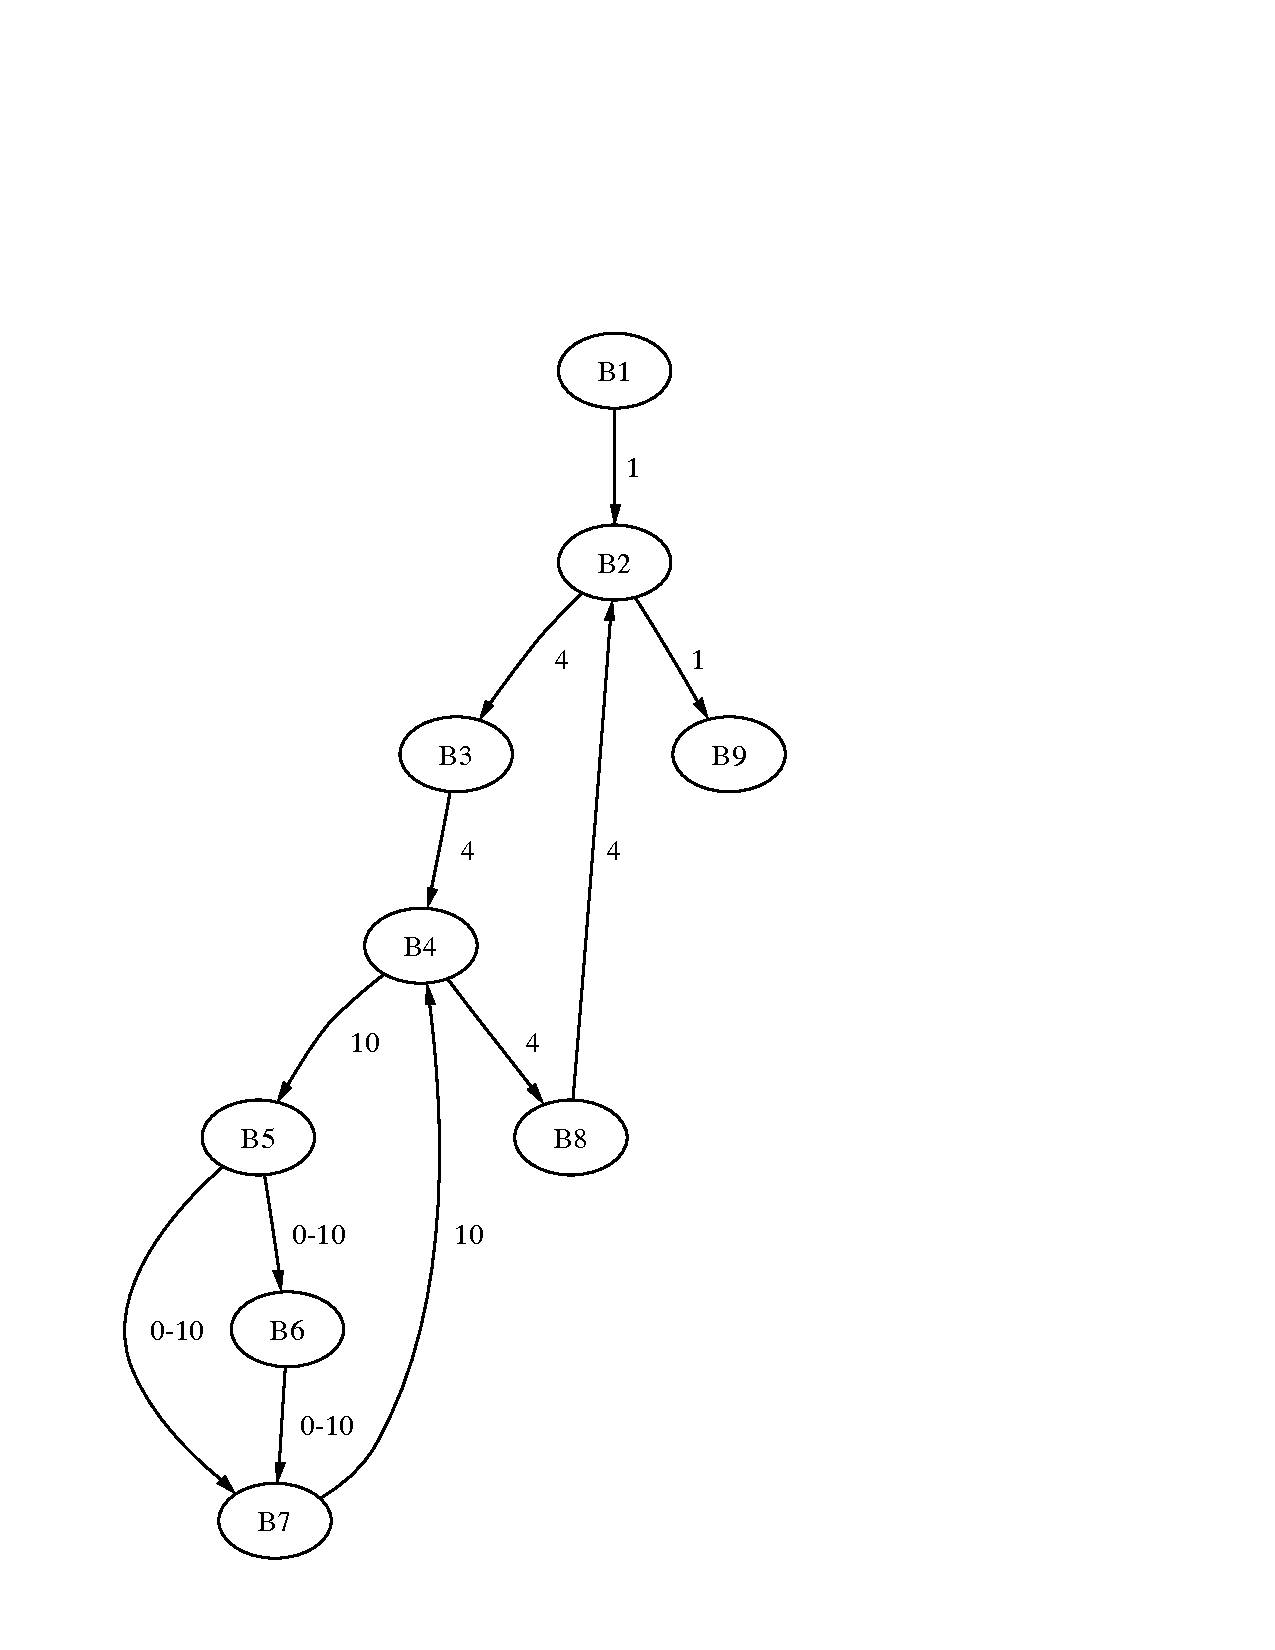
\includegraphics[height=\excelwidth]{results/results_wcet_cfg}
%    \caption{The control flow graph of the Bubble Sort example}
%    \label{fig:results:wcet:cfg}
%\end{figure}
%
%
%The values in the fifth and seventh columns (Count) of
%\tablename~\ref{tab:results:bubble:wcet} are derived from the CFG
%and show how often the basic blocks are executed in the worst and
%best cases. The WCET and BCET value for each block is calculated by
%multiplying the clock cycles by the execution frequency. The overall
%WCET and BCET values are calculated by summing the values of the
%individual blocks B1 to B8. The last block (B9) is omitted, as the
%measurement does not contain the return statement.
%
%The execution time of the program is measured using the cycle
%counter in JOP. The current time is taken at both the entry of the
%method and at the end, resulting in a measurement spanning from
%block B1 to the beginning of block B9. The last statement, the
%\code{return}, is not part of the measurement. The difference
%between these two values (less the additional 8 cycles introduced by
%the measurement itself) is given as the execution time in clock
%cycles (the last row in \tablename~\ref{tab:results:bubble:wcet}).
%The measured WCET and BCET values are exactly the same as the
%calculated values.
%
%In Figure~\ref{fig:results:wcet:sort}, the measured execution times
%for all 120 permutations of the input data are shown. The vertical
%axis shows the execution time in clock cycles and the horizontal
%axis the number of the test run. The first input sample is an
%already sorted array and results in the lowest execution time. The
%last sample is the worst-case value resulting from the reversely
%ordered input data. We can also see the 11 different execution times
%that result from executing basic block B6 (which performs the
%element exchange and takes 73 clock cycles) between 0 and 10 times.
%
%\begin{figure}
%    \centering
%    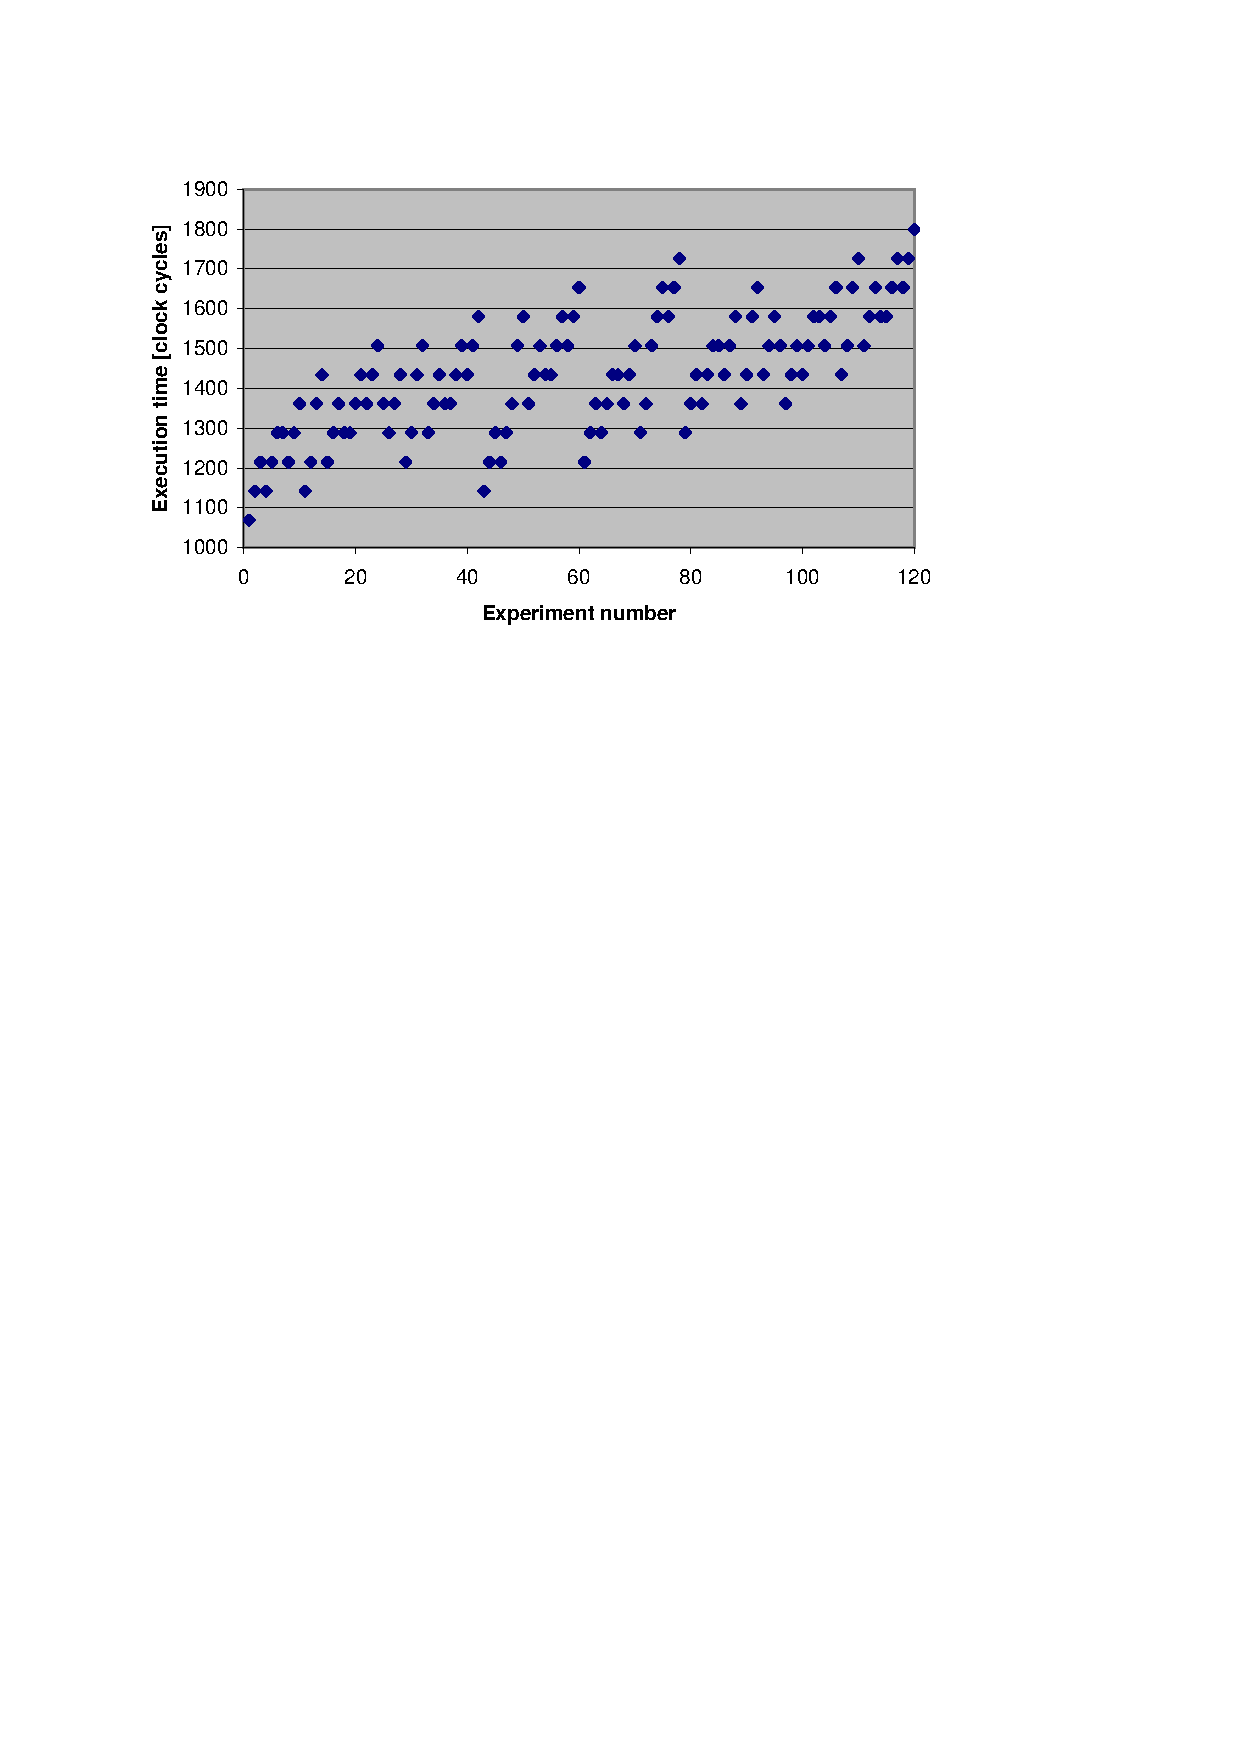
\includegraphics[width=\excelwidth]{results/results_wcet_sort}
%    \caption{Execution time in clock cycles of the Bubble Sort program}
%    \label{fig:results:wcet:sort}
%\end{figure}
%
%This example has demonstrated that JOP is a simple target for the
%WCET analysis. Most bytecodes have a single execution time (WCET =
%BCET), and the WCET of a task depends only on the control flow. No
%pipeline or data dependencies complicate the low-level part of the
%WCET analysis.
%
%%\subsection{Notes for targets}
%%
%%\subsubsection{JStamp}
%%
%%\begin{verbatim}
%%    aJile project in \usr2\ajile\bench
%%    Sources from JOP target
%%    LowLevel.java from directory aJile
%%    Remove .class in ...\dist\classes
%%    Generate .class with \bat\ajc.bat in source directory
%%        destination is ...\dist\classes
%%        e.g. in ...\src\bench: ajc jbe/DoAll
%%    aJile ChemBuilder (bench.ajp) use COM1 for System.out
%%    Terminal on Serial A, 9600 baud
%%        Did not get the System.out in Charade (but it worked some
%%        time ago)
%%    Charade: Reset, File-Load \usr2\ajile\bench\build.bin
%%\end{verbatim}


\section{Applications}
\label{sec:applications}

During the research for the PhD thesis, the first working version of
JOP was used in a real-world application. Using an architecture under
development in a commercial project entails risks. Nevertheless, this
was deemed to be the best way to prove the feasibility of the
processor. In this section, the experiences of the first project
involving JOP are summarized.

\subsection{Motor Control}
\label{sec:app:kfl}

In rail cargo, a large amount of time is spent on loading and
unloading of goods wagons. The contact wire above the wagons is the
main obstacle. Balfour Beatty Austria developed and patented a
technical solution, the so-called \emph{Kippfahrleitung}, to tilt up
the contact wire. This is done on a line up to one kilometer. An
asynchronous motor on each mast is used for this tilting. However, it
has to be done synchronously on the whole line.

Each motor is controlled by an embedded system. This system also
measures the position and communicates with a base station.
\figurename~\ref{fig:results:kfl:mast} shows the mast with the motor
and the control system in the `down' and `up' positions. The base
station has to control the deviation of individual positions during
the tilt. It also includes the user interface for the operator. In
technical terms, this is a distributed, embedded real-time control
system, communicating over an RS485 network.

\begin{figure}
    \centering
    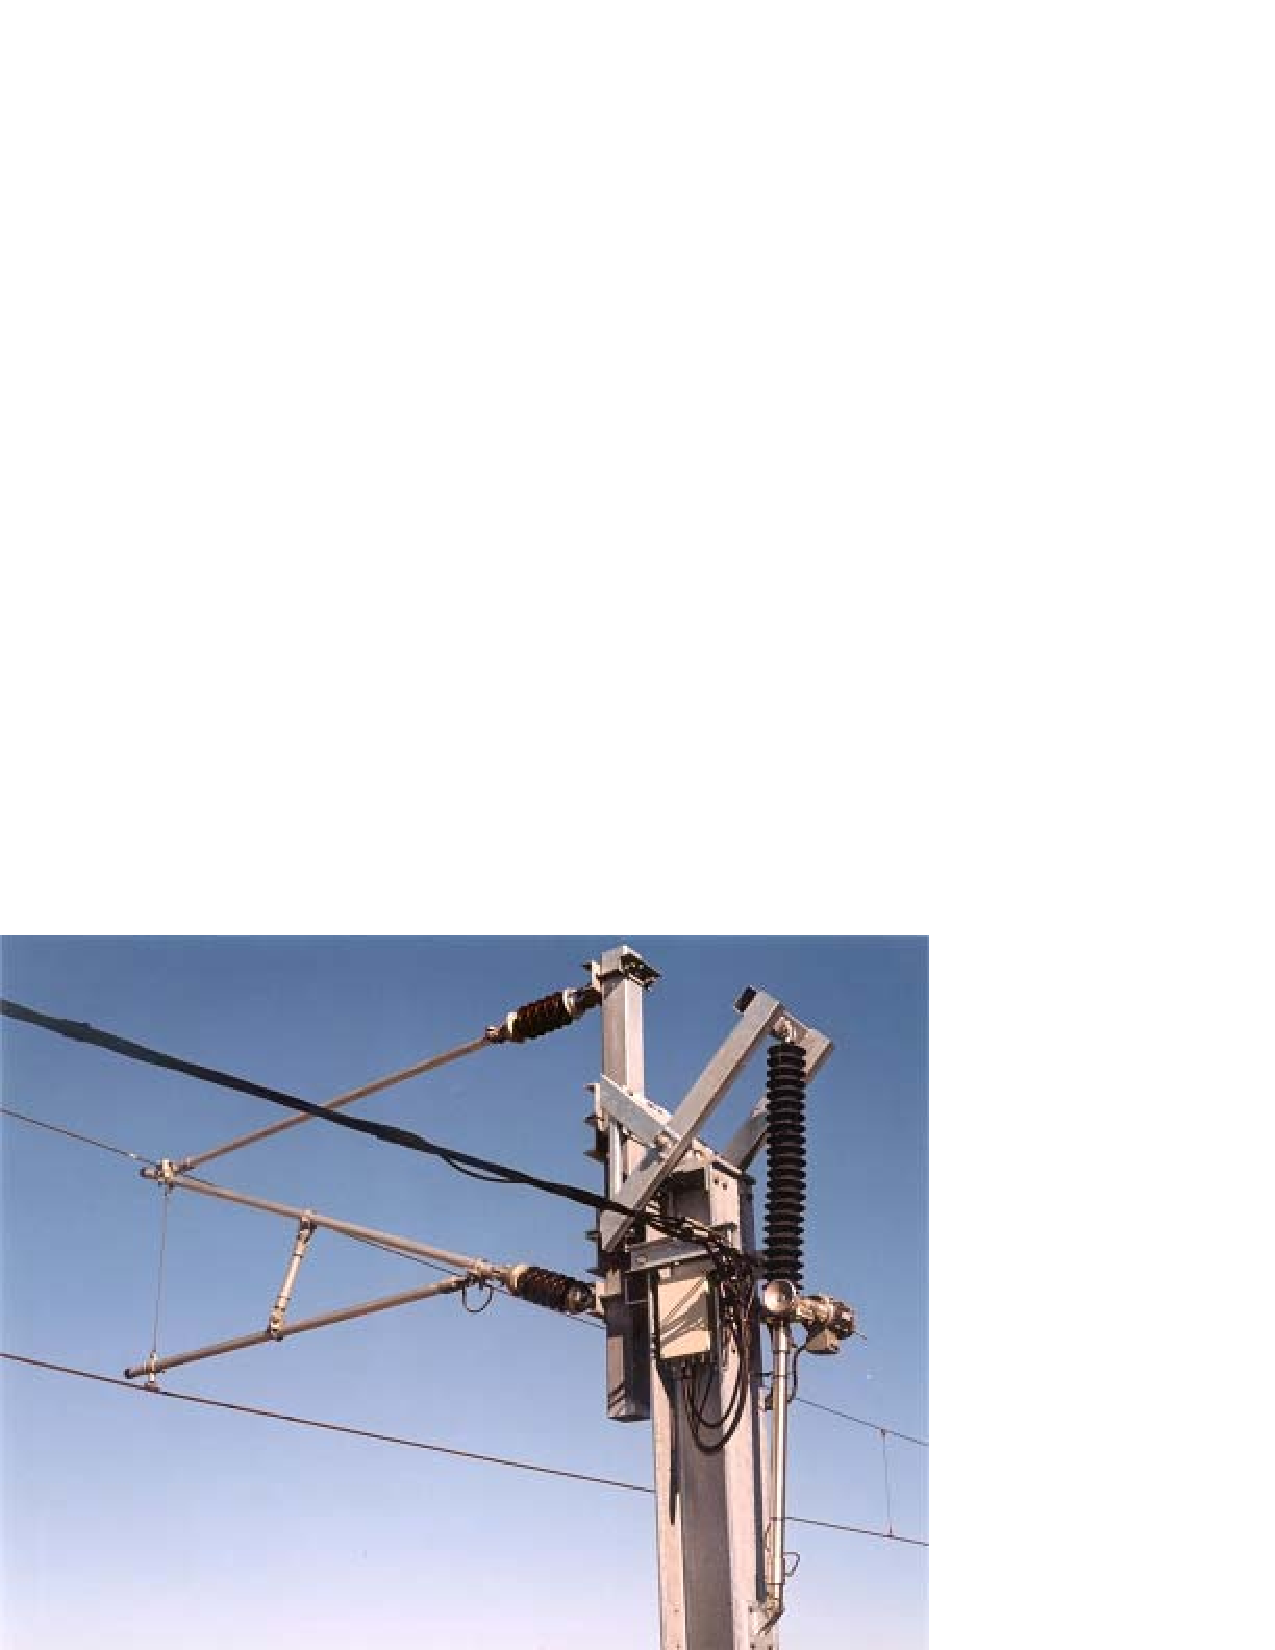
\includegraphics[width=7cm]{results/results_kfl_mast1}
    \hspace{1cm}
    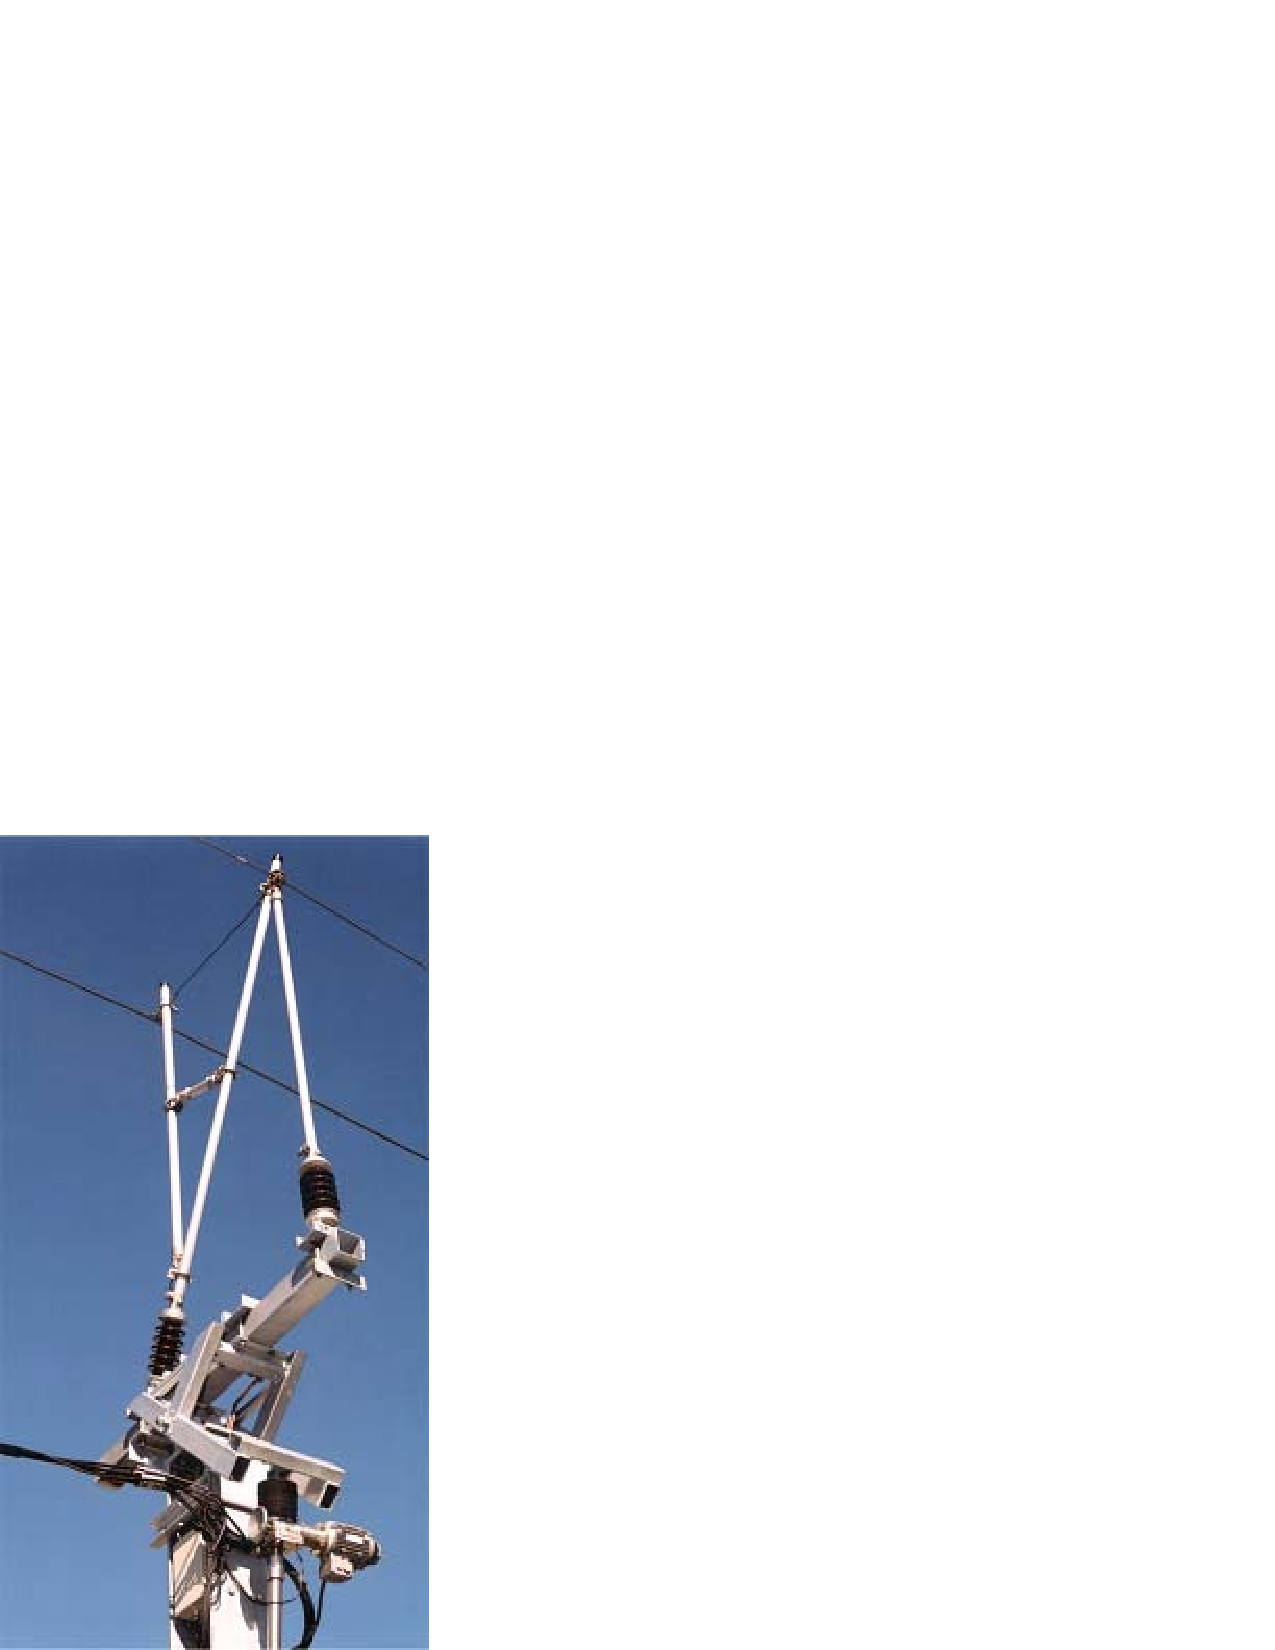
\includegraphics[width=4cm]{results/results_kfl_mast2}
    \caption{Picture of a \emph{Kippfahrleitung} mast in down and up position}
    \label{fig:results:kfl:mast}
\end{figure}

%\begin{figure}
%    \centering
%    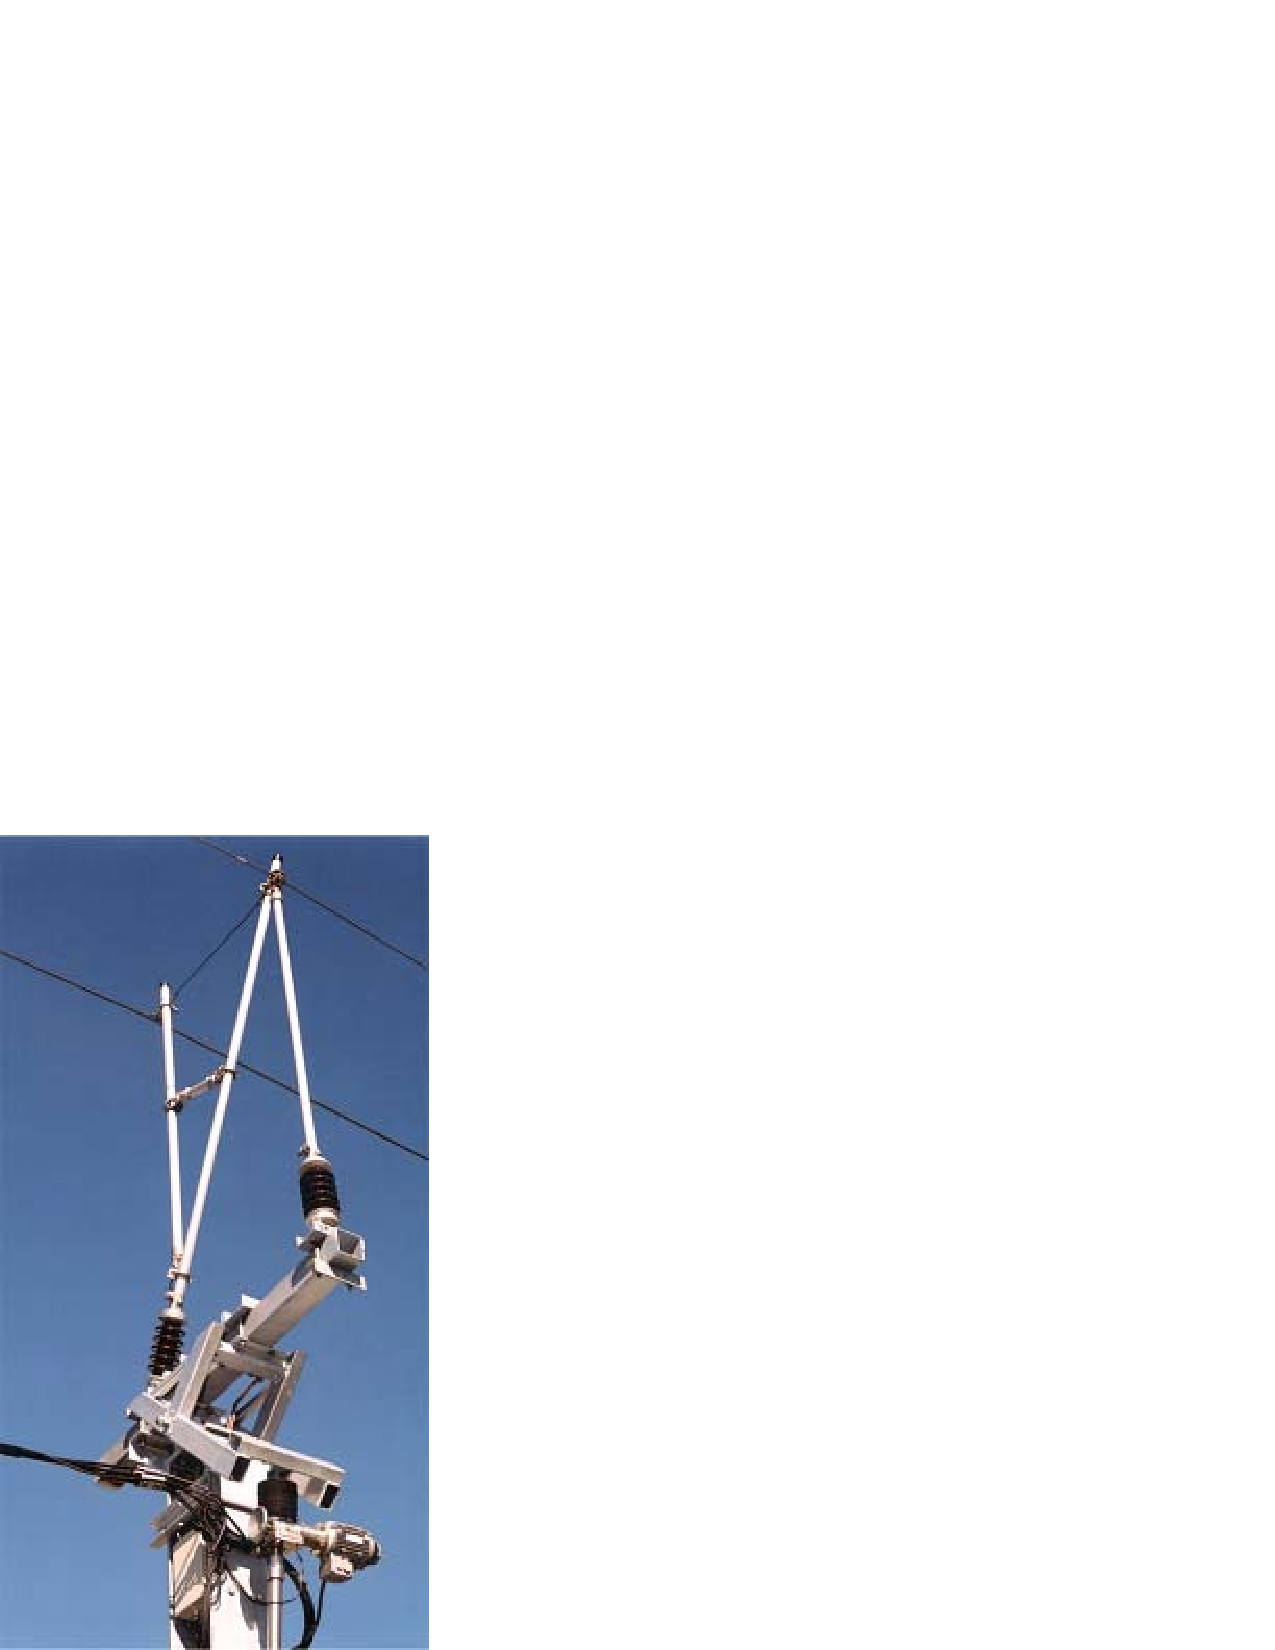
\includegraphics[width=4cm]{results/results_kfl_mast2}
%    \caption{Picture of the mast in up position}
%    \label{fig:results:kfl:mast2}
%\end{figure}


\subsubsection{Real Hardware}

Although this system is not mass-produced, there were nevertheless
cost constraints. Even a small FPGA is more expensive than a general
purpose CPU. To compensate for this, additional chips for the memory
and the FPGA configuration were optimized for cost. One standard
128KB Flash was used to hold FPGA configuration data, the Java
program and a logbook. External main memory was reduced to 128KB
with an 8-bit data bus.

To reduce external components, the boot process is a little
complicated. A watchdog circuit delivers a reset signal to a 32
macro-cell PLD. This PLD loads the configuration data into the FPGA.
When the FPGA starts, it disables the PLD and loads the Java program
from the Flash into the external RAM. After the JVM is initialized,
the program starts at \code{main()}.

The motor is controlled by silicon switches connected to the FPGA
with opto couplers. The position is measured with two end sensors and
a revolving sensor. The processor supervises the voltage and current
of the motor supply. A display and keyboard are attached to the base
station for the user interface. The communication bus (up to one
kilometer) is attached via an isolated RS485 data interface.

\subsubsection{Synthesized Hardware}

The following I/O modules were added to the JOP core in the FPGA:
%
\begin{itemize}
\item Timer
\item UART for debugging
\item UART with FIFO for the RS485 line
\item Four sigma delta ADCs
\item I/O ports
\end{itemize}
%
Five switches in the power line needed to be controlled by the
program. A wrong setting of the switches due to a software error
could result in a short circuit. Ensuring that this could not happen
was a straightforward task at the VHDL level. The sigma-delta ADCs
are used to measure the temperature of the silicon switches and the
current through the motor.

\subsubsection{Software Architecture}

The main task of the program was to measure the position using the
revolving sensor and communicate with the base station. This has to
be done under real-time constraints. This is not a very complicated
task. However, at the time of development, many features from a
full-blown JVM implementation, such as threads or objects, were
missing in JOP. The resulting Java was more like a \emph{tiny Java}.
It had to be kept in mind which Java constructs were supported by
JOP. Because there was no multi-threading capability, and in the
interests of simplicity, a simple infinite loop with constant time
intervals was used. Listing~\ref{lst:results:main} shows the
simplified program structure. After initialization and memory
allocation, this loop enters and never exits.

\begin{lstlisting}[float,caption=Simplified program structure,
label=lst:results:main]
    public static void main(String[] args) {

        init();
        Timer.start();
        forever();
        // this point is NEVER reached
    }

    private static void forever() {

        for (;;) {
            Msg.loop();
            Triac.loop();
            if (Msg.available) {
                handleMsg();
            } else {
                chkMsgTimeout();
            }
            handleWatchDog();
            Timer.waitForNextInterval();
        }
    }
\end{lstlisting}

\subsubsection{Communication}

Communication is based on a client-server structure. Only the base
station is allowed to send a request to a single mast station. The
station is then required to reply. The maximum reply time is bounded
by two time intervals. The base station handles timeout and retry. If
an irrecoverable error occurs, the base station switches off the
power to the mast stations, including the power supply to the motor.
This is the safe state of the whole system.

From the mast station perspective, every mast station supervises the
base station. The base station is required to send requests on a
regular basis. If this requirement is violated, the mast station
switches off its motor. The data is exchanged in small packets of
four bytes, including a one-byte CRC. To simplify the development,
commands to program the Flash in the mast stations and force a reset
were included. It is therefore possible to update the program, or
even change the FPGA configuration, over the network.

%\subsubsection{Benefits from using an FPGA}
%
%The flexibility of FPGAs made it possible to postpone some design
%decisions after production of the PCB. Since the production of the
%PBC was on the critical time line this helped to finish the complete
%project in time. During development, there have been situations
%where problems showed up that have not been foreseen.  Two examples
%are given where it was possible to find simple solutions:
%
%The routing of the PCB was almost finished. A question about cooling
%the switches (TRIAC) has arisen. The electronic development team
%insisted on a temperature sensor. The requirements in resolution and
%conversion time were low. A sigma-delta ADC with only two external
%passive components (a NTC thermistor and a capacitor) was
%implemented in the FPGA.
%
%When the sample rate for an ADC is low compared to the clock
%frequency of the digital system it is possible to transfer the AD
%conversion problem from the analogue to the time domain. In
%\figurename~\ref{fig_results_sigdel} the principle of a Sigma-Delta
%ADC is shown. Only the adder and the integrator have to be analogue
%components. A single bit DAC is just the FPGA digital output driving
%the signal between GND and VCCIO. The single bit ADC can be built
%with a comparator. For low resolution the threshold of the FPGA
%input is practical. The simplest form of an ADC built with an FPGA
%is shown in \figurename~\ref{fig_results_sigdel_real}. The filter
%averages $2^n$ samples and can be implemented as a counter.
%
%\begin{figure*}
%    \centering
%    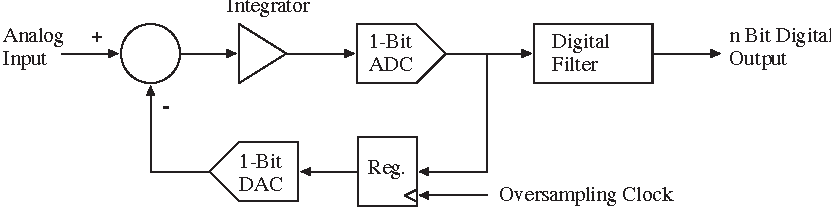
\includegraphics{results/results_sigdel}
%    \caption{A sigma-delta ADC}
%    \label{fig_results_sigdel}
%\end{figure*}
%
%
%\begin{figure*}
%    \centering
%    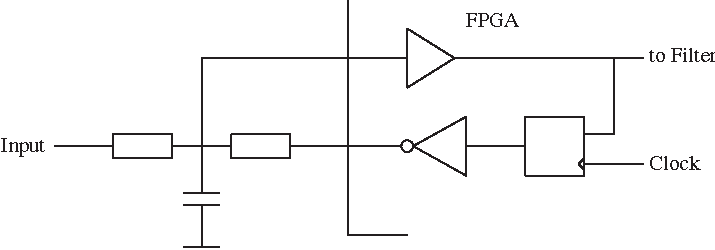
\includegraphics{results/results_sigdel_real}
%    \caption{A minimal sigma-delta ADC with an FPGA}
%    \label{fig_results_sigdel_real}
%\end{figure*}
%
%
%The AC current of the motor had to be monitored. The solution for
%this was a shunt resistor in every power line and an opto-coupler
%for isolation. However, it turned out that the shunt resistors got
%too hot and delivered to little voltage for the opto-couplers to
%work reliable. Having seen that it is possible to build an ADC in
%the FPGA a new idea was born. For EMC reasons, there is an inductor
%in every AC line. With a few windings of wire, a simple transformer
%can be built. The resulting voltage was amplified, rectified and
%used for current measurement. An additional comparator was used for
%an exacter threshold than the input buffer of the FPGA. This
%solution kept the board cool and added extra functionality. It is
%now possible to define two thresholds for too little and too much
%current.
%

\subsection{Further Projects}

TAL, short for TeleAlarm, is a remote tele-control and data logging
system. TAL communicates via a modem or an Ethernet bus with a SCADA
system or via SMS with a mobile phone. For this application, a
minimal TCP/IP stack needed to be implemented. This stack was the
reason for implementing threads and a simple real-time system in
JOP.

Another application of JOP is in a communication device with soft
real-time properties -- Austrian Railways' (\"OBB) new security
system for single-track lines. Each locomotive is equipped with a GPS
receiver and a communication device. The position of the train,
differential correction data for GPS, and commands are exchanged with
a server at the central station over a GPRS virtual private network.
JOP is the heart of the communication device in the locomotive. The
flexibility of the FPGA and an Internet connection to the embedded
system make it possible to upgrade the software and even the
processor in the field.


\section{Summary}

In this chapter, we presented an evaluation of JOP. We have seen
that JOP is the smallest hardware realization of the JVM available
to date. Due to the efficient implementation of the stack
architecture, JOP is also smaller than a \emph{comparable} RISC
processor in an FPGA. Implemented in an FPGA, JOP has the highest
clock frequency of all known Java processors.

We compared JOP against several embedded Java systems and, as a
reference, with Java on a standard PC. A Java processor is up to 500
times faster than an interpreting JVM on a standard processor for an
embedded system. JOP is about six times faster than the aJ80 Java
processor and as fast as the aJ100\footnote{The measured aJ100
system contained faster SRAMs than the FPGA board for JOP.}.
Preliminary results using compiled Java for a RISC processor in an
FPGA, with a similar resource usage and maximum clock frequency to
JOP, showed that native execution of Java bytecodes is faster than
compiled Java.

We compared the basic properties of the real-time scheduler on JOP
against the RTSJ implementation on Linux. The integration of the
scheduler in the JVM, and the timer interrupt under scheduler
control, results in an efficient platform for Java in embedded
real-time systems. JOP performs better and more predictably than the
reference implementation of the RTSJ under Linux.

We also performed WCET analysis of the implemented JVM at the
microcode level. This analysis provides the WCET and BCET values for
the individual bytecodes. We have also shown that there are no
dependencies between individual bytecodes. This feature, in
combination with the method cache (see Section~\ref{sec:cache}),
makes JOP an easy target for low-level WCET analysis of Java
applications.

Usage of JOP in three real-world applications showed that the
processor is mature enough to be used in commercial projects.


%\bibliographystyle{plain}
%\bibliography{../bib/mybib}
%\end{document}
